\documentclass[english]{../thermomemo/thermomemo}
% NOTE: You must pass either norsk or english as an option!
\usepackage[utf8]{inputenc}

\title{Implementation and testing of the Lee-Kesler equation of state in ThermoPack}
\author{J\o rgen R\o ysland Aarnes}

\usepackage[normalem]{ulem}
\usepackage{hyperref}
\usepackage{color}
\usepackage{amsmath}
\usepackage{graphicx}
%\usepackage[norsk]{babel}
\usepackage{setspace}
\usepackage{float}
%\newcommand{\HRule}{\rule{\linewidth}{0.5mm}}
\numberwithin{equation}{section}
\usepackage{mathtools}
\usepackage{rotating}
\usepackage{verbatim}

\newcommand*{\pd}[2]{\frac{\partial #1}{\partial #2}}
\newcommand*{\pdd}[2]{\frac{\partial^2 #1}{\partial #2^2}}
\newcommand*{\pder}[2]{\left(\frac{\partial #1}{\partial #2}\right)}
\newcommand*{\pdder}[2]{\left(\frac{\partial^2 #1}{\partial #2^2}\right)}
\newcommand*{\pdcross}[3]{\left(\frac{\partial^2 #1}{\partial #2 \partial #3}\right)}
\newcommand*{\reff}[1]{(\ref{#1})}



\definecolor{midnightblue}{RGB}{35,35,132}
\definecolor{urlblue}{RGB}{70,130,180}

\hypersetup{
    colorlinks=true,
    linkcolor=midnightblue,
    urlcolor=urlblue,
    citecolor=midnightblue,
    linktoc=page
}

\usepackage[activate={true,nocompatibility},final,kerning=true,tracking=true,spacing=true,stretch=10,shrink=10]{microtype}
\microtypecontext{spacing=nonfrench}
\SetExtraKerning[unit=space]
    {encoding={*}, family={bch}, series={*}, size={footnotesize,small,normalsize}}
    {\textendash={400,400}, % en-dash, add more space around it
     "28={ ,150}, % left bracket, add space from right
     "29={150, }, % right bracket, add space from left
     \textquotedblleft={ ,150}, % left quotation mark, space from right
     \textquotedblright={150, }} % right quotation mark, space from left
\SetTracking{encoding={*}, shape=sc}{0}

\graphicspath{{gfx/}}

\begin{document}
\frontmatter

\tableofcontents

\section{Introduction}
This document is meant to provide complete documentation for the Lee-Kesler package for ThermoPack, developed by the author during his stay as a summer intern during June and July 2013 at SINTEF Energy Research. To this end, the complete theoretical framework, derived from the equations and relations presented in the original articles \cite{LK} and \cite{PKP}, is included in this text.

The main difference between the original article and this implementation, is the following: The original approach is rather straightforward: All thermodynamic properties are calculated by some relation with the compressibility factor. This yields rather complicated expressions for the thermodynamic properties, but since these are derived in \cite{LK}, their implementation is trivial. However, consistency checks and calculations not presented in this article require a lot of work to derive, since the expressions get really messy when differentiated further. The implementation presented here is based on a powerful, modern method, deriving all thermodynamic properties of interest from the reduced residual Helmholtz free energy function, $F$. This method is thoroughly discussed in \cite{MM}.

All implementation is done using FORTRAN 90, and compiled with GFortran. Plots have been made in GNU Plot. No code is presented in this document.  

\section{General theory}
This section is an introductory section to establish the general theory used to derive the theoretical framework for the implementation of the Lee-Kesler method. This theory can be found in much more detail in \cite{MM}.
\subsection{Thermodynamic properties of interest}

The thermodynamic properties of interest are the compressibility factor, the entropy, the enthalpy and the fugacity coefficients in the mixture. To express these, the internal energy, the Helmholtz free energy and the fugacity is also introduced in this subsection.

\subsubsection*{Compressibility factor}
The compressibility factor is a measure of how much the thermodynamic properties of a real fluid deviates from those expected of an ideal fluid. Mathematically it is the ratio of the molar volume of a real gas to the molar volume predicted by the ideal gas law at the same temperature and pressure.

\begin{equation}
\label{def:z}
z = \frac{v}{v_{ig}} = \frac{Pv}{RT} = \frac{PV}{nRT}
\end{equation}

In the equation above, $z$ is the compressibility factor, $v = V/n$ is the specific volume (molar volume), $v_{ig}$ is the specific volume of an ideal gas, $R$ is the gas constant, and P, V, T and n are pressure, volume, temperature and number of moles of the fluid, respectively. Hence, if $z = 1$, the fluid has ideal gas behaviour.

\subsubsection*{Internal energy}
The internal energy is defined as:
\begin{equation}
\label{def:U}
U(S,V,\textbf{n}) = ST - PV + \sum_i n_i \mu _i
\end{equation}

where $S$ is the entropy, $\textbf{n}$ is the composition vector, and $n_i$ and $\mu _i$ are the the number of moles and chemical potential of component $i$ in a mixture, respectively. The exact differential form of Equation \reff{def:U}, given its independent variables, is

\begin{equation}
\label{def:dU}
\mathrm{d}U  = T\mathrm{d}S - P \mathrm{d}V - \sum_i \mu_i \mathrm{d}n_i
\end{equation}

\subsubsection*{Helmholtz free energy}
The Helmholtz free energy is defined as:
\begin{equation}
\label{def:A}
A(T,V,\textbf{n}) = U - TS
\end{equation}

By using equation \reff{def:dU}, the differential form of the Helmholtz free energy is given by:
\begin{equation}
\label{def:dA}
dA = -SdT - PdV -  \sum_i \mu_i \mathrm{d}n_i
\end{equation}

Taking the partial derivative of the Hemlholtz free energy, with respect to volume, Equation \reff{def:dA} yields:
\begin{equation}
\label{def:-P}
\pder{A}{V}_{T,\textbf{n}} = -P
\end{equation}

Hence, if an equation of state is given as an explicit pressure equation, such that $P = P(T,V,\textbf{n})$, Helmholtz free energy might be found by integration. How this is done will be discussed later in this section.

\subsubsection*{Entropy}
By using Equation \reff{def:A}, the entropy may be defined in terms of the Helmholtz free energy, by taking its the partial derivative with respect to temperature:
\begin{equation}
\label{def:S}
S = - \pder{A}{T}_{V,\textbf{n}}
\end{equation}

\subsubsection*{Enthalpy}
The enthalpy is defined as:
\begin{equation}
\label{def:H1}
H(S,P,\textbf{n}) = U + PV
\end{equation}

By inserting Equation \reff{def:A} into \reff{def:H1} the enthalpy can be expressed in a more convenient form:
\begin{equation}
\label{def:H2}
H = A + TS + PV
\end{equation}

\subsubsection*{Fugacity and fugacity coefficients}
For a pure ideal gas, the change in chemical potential corresponding to a change in pressure, at a constant temperature, is given by:
\begin{equation}
\label{eq:P/P0}
RT \ln \frac{P}{P_0} = \mu^{ig} (T,P) - \mu^{ig} (T, P_0)
\end{equation}

where $\mu^{ig} (T,P)$ is the ideal gas chemical potential, at temperature $T$ and pressure $P$. As real fluids do not behave like perfect gasses, Equation \reff{eq:P/P0} is generalized by defining the thermodynamic property known as the fugacity. The defining equation is:
\begin{equation}
\label{eq:fugacity}
RT \ln \frac{f(T,P)}{P_0} = \mu (T,P) - \mu^{ig} (T, P_0)
\end{equation}

where $f = f(T,P)$ is the fugacity. It is more convenient to work with the fugacity coefficient, rather than the fugacity, which for a pure component is defined as $\phi = f/P$. For a mixture, the fugacity component, as well as the fugacity, is dependent on the composition of the fluid. The fugacity coefficient for component $i$ is related to the fugacity of the same component by $\phi = f_i/P x_i$, where $x_i$ is the mole fraction of component $i$. Without further derivation (for detail, see \cite{MM}), the fugacity coefficients in a mixture are given by:
\begin{equation}
\label{def:lnphi}
\ln \phi_i (T,P,\textbf{n}) = \frac{1}{RT} \pder{A^R}{n_i}_{T,V} - \ln z
\end{equation}

\subsection{Residual properties}
An arbitrary thermodynamic property $M$,  may be represented as a sum of an ideal contribution, and a so called residual contribution:
\begin{align}
\label{def:M(T,V,n)}
& M = M^{ig}(T,V,\textbf{n}) + M^R(T,V,\textbf{n}) \\
\label{def:M(T,P,n)}
& M = M^{ig}(T,P,\textbf{n}) + M^R(T,P,\textbf{n}) 
\end{align}
where the superscript large R denotes the residual quantity (the choice of notation upper case R, instead of the commonly used lower case r, is to avoid confusion between \textit{residual} values and \textit{reduced} values, with subscript lower case r). Hence, a residual property is the difference between the a real gas property and an ideal gas property.

Equations \reff{def:M(T,V,n)} and \reff{def:M(T,P,n)} are basically the same equation, differing only in dependence on volume or pressure. It may seem unnecessary  to separate the two, since volume and pressure are not independent variables, but unlike the thermodynamic property at hand, the value of the residual property changes with a variable change. The difference in the two sets of residual properties is due to the difference in the hypothetical ideal gas properties at the two states $(T,V,\textbf{n})$ and $(T,P,\textbf{n})$, respectively. An example of this is the residual Helmholtz energy, where:
\begin{equation}
\label{eq:A^R(T,V,n)-A^R(T,P,n)}
A^R(T,V,\textbf{n}) - A^R(T,P,\textbf{n}) = nRT \ln z
\end{equation}

If the partial derivatives of the real and ideal thermodynamic property, with respect to volume or pressure is known, the residual property can be calculated by:
\begin{align}
\label{def:M^R(T,V,n)}
& M^R(T,V,\textbf{n}) = \int_\infty ^V \left(\pder{M(T,V',\textbf{n})}{V'}_{T,\textbf{n}} - \pder{M^{ig}(T,V',\textbf{n})}{V'}_{T,\textbf{n}} \right) \mathrm{d}V' \\
& M^R(T,P,\textbf{n}) = \int_0 ^P \left(\pder{M(T,P',\textbf{n})}{P'}_{T,\textbf{n}} - \pder{M^{ig}(T,P',\textbf{n})}{P'}_{T,\textbf{n}} \right) \mathrm{d}P'
\label{def:M^R(T,P,n)}
\end{align}

\subsubsection*{Departure functions}
The residual value of a thermodynamic property is often of as great, if not greater interest than the real value. This is due to the fact that experimentally, measuring changes in an extensive property is much more convenient, than measuring absolute values with an arbitrary mean. Thermodynamic properties like entropy and enthalpy are often represented as so called departure functions, that basically are scaled versions of the residual values.
\subsection{The reduced residual Helmholtz function}
One such thermodynamic property, for which the partial derivative with respect to volume is often known, is the Helmholtz free energy. If an equation of state can be formulated as an explicit pressure equation, the residual Helmholtz free energy can be derived analytically by:
\begin{equation}
\label{def:A^R1}
A^R(T,V,\textbf{n}) = \int_\infty ^V \left(\pder{A}{V'}_{T,\textbf{n}} - \pder{A^{ig}}{V'}_{T,\textbf{n}} \right) \mathrm{d}V' \\
\end{equation}

By inserting Equation \reff{def:-P} into \reff{def:A^R1}, and further by using Equation \reff{def:z} to express the real fluid pressure, Equation \reff{def:A^R1} can be rewritten to:

\begin{equation}
\label{def:A^R2}
A^R(T,V,\textbf{n}) = - \int_\infty ^V \left(P - P^{ig} \right) \mathrm{d}V'  = - nRT \int_\infty ^V \frac{1}{V'} (z-1) \mathrm{d}V'
\end{equation}

A more convenient function to work with, rather than the residual Helmholtz free energy, is the reduced residual Helmholtz function $F$, defined as:

\begin{equation}
\label{def:F}
F(T,V,\textbf{n}) = \frac{A^R(T,V,\textbf{n})}{RT} = - n \int_\infty ^V \frac{1}{V'} (z-1) \mathrm{d}V'
\end{equation}

Now that the reduced residual Helmholtz function is defined, it is of great benefit to express all the thermodynamic properties of interest, and their derivatives in, terms of $F$, and its derivatives. This is a very powerful approach, since it relates a lot of expressions to a single function. Rather than calculating many different properties (entropy, enthalpy, etc.) from the equation of state, only the function $F$ and its derivatives are calculated, and the rest follows almost without any cost. By combining Equation \reff{def:F} with Equations \reff{def:S}, \reff{def:H2} and \reff{def:lnphi}, respectively, the following equations are found:

\begin{align}
\label{def:S^R(T,V,n)}
& S^R(T,V,\textbf{n}) = -R \left[F + T \pder{F}{T}_{V,\textbf{n}} \right] \\
\label{def:H^R(T,P,n)}
& H^R(T,P,\textbf{n}) = - RT \pder{F}{T}_{V,\textbf{n}} + PV - nRT \\
\label{def:lnphi(T,P,n)}
& \ln \phi_i (T,P,\textbf{n}) = \pder{F}{n_i}_{T,V} - \ln z
\end{align}

The compressibility factor may also be expressed in terms of $F$, by differentiating and rearranging Equation \reff{def:F}. However, the initial expression for $z$, given by Equation \reff{def:z} is simple enough as it is, being only dependent on temperature, pressure, volume and compositions.
\\ \\
In most thermodynamic experiments, it is easier to both vary and measure temperature and pressure, than volume. Therefore, all thermodynamic properties should be calculated for $(T,P,\textbf{n})$-states. The residual entropy may be found for the $(T,P,\textbf{n})$-state, by combining Equations \reff{def:S^R(T,V,n)} and \reff{eq:A^R(T,V,n)-A^R(T,P,n)}:
\begin{equation}
\label{def:S^R(T,P,n)}
S^R(T,P,\textbf{n}) = S^R(T,V,\textbf{n}) +nR \ln z
\end{equation}

\subsubsection*{Departure functions of entropy and enthalpy}
Now that the residual values of the entropy and the enthalpy are defined, their departure functions can be expressed by:
\begin{align}
& S_{dep} = \frac{S^R(T,P,\textbf{n})}{R} \\
& H_{dep} = \frac{H^R(T,P,\textbf{n)}}{R T_c}
\end{align}
where $T_c$ is the critical temperature of the fluid at hand. If the fluid is a mixture, this should be represented by the critical mixing temperature, $T_{cM}$, defined by some mixing rules.
\subsection{Partial derivatives of the thermodynamic properties}

\subsubsection*{Pressure}
To simplify the notation in the following derivatives, a relation between the pressure and its derivatives, and the reduced residual Helmholtz function is introduced. By inserting Equation \reff{def:F} into Equation \reff{def:-P}, the pressure can be related to the reduced residual Helmholtz function by:

\begin{equation}
\label{def:P}
P(T,V,\textbf{n}) = -RT \left( \frac{\partial F}{\partial V} \right)_{T, \textbf{n}} + \frac{nRT}{V}
\end{equation}

The partial derivatives of the pressure, with respect to temperature, volume and composition, respectively, are given by:
\begin{align}
\label{eq:P_T}
& \pder{P}{T}_{V, \textbf{n}} = \frac{P}{T} - RT \pdcross{F}{T}{V}_{n_i} \\
\label{eq:P_V}
& \pder{P}{V}_{T, \textbf{n}} = -RT \pdder{F}{V}_{T, \textbf{n}} - \frac{nRT}{V^2} \\
\label{eq:P_i}
& \pder{P}{n_i}_{T,V} = -RT \pdcross{F}{n_i}{V}_T + \frac{RT}{V}
\end{align}

Further, the partial derivatives of the volume with respect to composition and temperature are defined, by the use of the triple product rule and the derivatives of the pressure (see Appendix \ref{app:tripProdRule} for details):
\begin{align}
\label{def:V_i}
\bar{V}_i \equiv \pder{V}{n_i}_{T,P} =  - \frac{\pder{P}{n_i}_{T,V}}{\pder{P}{V}_{T,\textbf{n}}} \\
\label{def:V_T}
\bar{V}_T \equiv \pder{V}{T}_{P,\textbf{n}} =  - \frac{\pder{P}{T}_{V,\textbf{n}}}{\pder{P}{V}_{T,\textbf{n}}}
\end{align}

The following derivatives are all done for functions that are $(T,P,\textbf{n})$-states, that is $z = z(T,P,\textbf{n})$, $S^R = S^R(T,P,\textbf{n})$, $H^R = H^R(T,P,\textbf{n})$ and $\ln \phi_i = \ln \phi_i(T,P,\textbf{n})$. Several of these calculations get rather technical, and only the resulting expressions are presented here. For the complete derivation, see Appendix \ref{app:partDerivatives}.
\subsubsection*{Compressibility}
\begin{align}
\label{eq:z_T}
& \left( \frac{\partial z}{\partial T} \right)_{P, \textbf{n}} = -z\left[\frac{1}{T} - \frac{\bar{V}_T}{V}\right] \\
\label{eq:z_P}
& \left( \frac{\partial z}{\partial P} \right)_{T, \textbf{n}} = z \left[ \frac{1}{P} + \frac{1}{V \pder{P}{V}_{T,\textbf{n}}} \right] \\
\label{eq:z_i}
& \left( \frac{\partial z}{\partial n_i} \right)_{T,P} = - z \left[ \frac{1}{n} - \frac{\bar{V}_i}{V}  \right]
\end{align}

\subsubsection*{Entropy}
\begin{align}
\label{eq:S^R_T}
& \pder{S^R(T,P,\textbf{n})}{T}_{P,\textbf{n}} = \bar{V}_T \pder{P}{T}_{V,\textbf{n}} - R \left[2\pder{F}{T}_{V,\textbf{n}} + T \pdder{F}{T}_{V,\textbf{n}} + \frac{n}{T} \right] \\
\label{eq:S^R_P}
& \pder{S^R(T,P,\textbf{n})}{P}_{T,\textbf{n}} = \frac{nR}{P} - \bar{V}_T \\
\label{eq:S^R_i}
& \pder{S^R(T,P,\textbf{n})}{n_i}_{T,P} = \bar{V}_i \pder{P}{T}_{V,\textbf{n}} - R\left[ \pder{F}{n_i}_{T,V} + T\pdcross{F}{T}{n_i}_V + 1 - \ln z \right] 
\end{align}

\subsubsection*{Enthalpy}
\begin{align}
\label{eq:H^R_T}
& \pder{H^R}{T}_{P, \textbf{n}} = \bar{V}_T T \pder{P}{T}_{V,\textbf{n}} - RT \left[ 2\pder{F}{T}_{V,\textbf{n}} + T \pdder{F}{T}_{V,\textbf{n}} + \frac{n}{T} \right] \\
\label{eq:H^R_P}
& \pder{H^R}{P}_{T, \textbf{n}} = V - T \bar{V}_T \\
\label{eq:H^R_i}
& \pder{H^R}{n_i}_{T,P}  = \bar{V}_i T \pder{P}{T}_{V,\textbf{n}} -RT^2 \pdcross{F}{T}{n_i}_V - RT
\end{align}

\subsubsection*{Fugacity coefficients}
\begin{align}
\label{eq:lnphi_T}
& \pder{\ln \phi_i}{T}_{P, \textbf{n}} = \pdcross{F}{T}{n_i}_V + \frac{1}{T} - \frac{\bar{V}_i}{RT}  \pder{P}{T}_{V,\textbf{n}} \\
\label{eq:lnphi_P}
& \pder{\ln \phi_i}{P}_{T, \textbf{n}} = \frac{\bar{V}_i}{RT} - \frac{1}{P} \\
\label{eq:lnphi_i}
& \pder{\ln \phi_i}{n_j}_{T, P}  = \pdcross{F}{n_j}{n_i}_{T,P} + \frac{1}{n} + \frac{\pder{P}{V}_{T,\textbf{n}}}{RT} \bar{V}_j \bar{V}_i 
\end{align}

\subsection{Consistency tests}
\label{subsec:consistCheck}
As the previous subsection demonstrates, the partial derivatives of the thermodynamic properties of interest get quite messy. Therefore, it is essential to be able to test if these calculations are correct, when implementing them on a computer. Two ways to test these derivatives are presented here.

\subsubsection*{Numerical evaluation of derivatives}
All analytical derivatives should be tested with comparison to their numerical counterparts. This may seem straightforward, and for the most part it is, but one may run into problems when testing the partial derivatives without taking care to ensure that the correct variables are held constant at the correct time. 

As an example of this, consider the partial derivatives of residual entropy, Equations \reff{eq:S^R_T} - \reff{eq:S^R_i}. By writing a routine that takes temperature, pressure and composition as input, and calculates the residual entropy, and its derivatives, the correct comparison can be made. The volume is not held constant in any of the derivatives, and must be calculated from an equation of state in the routine.

By contrast, if the partial derivatives of the pressure are to be tested, the routine written for the residual entropy, extended to include the pressure derivatives, will not yield the correct result. This is because the pressure is a function of temperature, \textit{volume} and composition, hence these variables must be inputs to the routine, while the pressure must be calculated from the equation of state.

A recommended way to compare the numerical derivatives to the analytical ones is to first write a routine that takes temperature volume and composition as inputs, and test the partial derivatives of the pressure and the reduced residual Helmholtz function (both of these are given for the $(T,V,\textbf{n})$-state). When the correctness of these are ensured, a new routine may be written, that test the partial derivatives thermodynamic properties given by Equations \reff{eq:z_T} - \reff{eq:lnphi_i}.

Numerical partial derivatives for a function $M = M(x,y)$ of first and second order are given by:
\begin{align}
  \phantom{\frac{\partial^2 M}{\partial x \partial y}}
    \label{eq:numDir1}
	\pd{M}{x} & = \frac{M(x + \delta x,y) - M(x ,y)}{\delta x } \\
	\pd{M}{y} & = \frac{M(x ,y+ \delta y) - M(x ,y)}{\delta y } \\
	\pdd{M}{x} & = \frac{M(x + \delta x,y) - 2 M(x ,y) + M(x - \delta x,y)}{2 \delta x} \\
	\pdd{M}{y} & = \frac{M(x ,y+ \delta y) - 2 M(x ,y) + M(x ,y- \delta y)}{2 \delta y} \\
  & \begin{aligned}
    \label{eq:numDir5}
    \mathllap{\frac{\partial^2 M}{\partial x \partial y}}
	 & = \frac{1}{4 \delta x \delta y} [M(x + \delta x,y + \delta y)- M(x + \delta x,y - \delta y) \\
	 & \qquad \qquad - M(x - \delta x,y + \delta y) + M(x - \delta x,y - \delta y) ]
  \end{aligned}
\end{align}

where $\left| \dfrac{\partial x}{x} \right| \ll 1$,  $\left|\dfrac{\partial y}{y} \right| \ll 1$.
 
\subsubsection*{Identities}  
In addition to the numerical test of the derivatives, thermodynamic identities and identities found from Euler's theorem, serve as decent consistency tests for the analytical derivatives. The test supplied here are all found in \cite{MM}. To test the derivatives of the reduced residual Helmholtz function, the following identities may be applied:
\begin{align}
\label{test:1}
& F = V \pder{F}{V}_{T,\textbf{n}} + \sum_i n_i \pder{F}{n_i}_{T,V} \\
\label{test:2}
& V \pdcross{F}{V}{n_i}_T + \sum_j n_j \pdcross{F}{n_j}{n_i}_{T,V} = 0 \\
\label{test:3}
& V \pdder{F}{V}_{T,\textbf{n}} + \sum_j n_j \pdcross{F}{n_j}{V}_T = 0
\end{align}

When these are all satisfied, the fugacity coefficients and their derivatives may be tested by the identities:
\begin{align}
\label{test:4}
& \left( \frac{\partial}{\partial n_j} \sum_i n_i \ln \phi_i \right)_{T,P} = \ln \phi_j \\
\label{test:5}
& \pder{\ln \phi_i}{n_j}_{T,P} = \pder{\ln \phi_j}{n_i}_{T,P} \\
\label{test:6}
& \sum_i n_i \pder{\ln \phi_i}{n_j}_{T,P} = 0 \\
\label{test:7}
& \left( \frac{\partial}{\partial P} \sum_i n_i \ln \phi_i \right)_{T,\textbf{n}} = \frac{(z-1) n}{P} \\
\label{test:8}
& \sum_i n_i \pder{ \ln \phi_i}{T}_{P,\textbf{n}} = -\frac{H^R(T,P,\textbf{n})}{RT^2}
\end{align}

\section{The Lee-Kesler model}
\subsection{Simple fluid, reference fluid}
\label{sec:simpRef}
The Lee-Kesler equation of state is a two fluid corresponding state method. This means that all thermodynamic properties are calculated twice, once for a simple fluid, and once for a reference fluid. These two solutions are then combined, to give the result for the fluid at hand, by the following equation:
\begin{equation}
\label{eq:LK_main}
M = M^{(0)} + \frac{\omega_M}{\omega^{(r)}}(M^{(r)} - M^{(0)})
\end{equation}
where $M$ is the thermodynamic property to be found, $M^{(0)}$ and $M^{(r)}$ is this property for the simple fluid and reference fluid, respectively, $\omega_M$ is the acentric factor for the mixture (if the fluid is a pure fluid this is equal to the acentric factor of the pure fluid) and $\omega^{(r)} = 0.3978$ is the acentric factor of the reference fluid. Equation \reff{eq:LK_main} is valid for $M = z$, $S^R$, $H^R$, $G^R$, etc. The solution for $M$ may be viewed as an average between the simple and the reference fluid, weighted regarding to how similar the fluid is to each of them.

The parameters that dictate whether the calculations are done for the simple fluid or the reference fluid are a two sets of constants in the equation of state. One set for the simple fluid and one set for the reference fluid. These have been found by calculations on methane as simple fluid, and n-Octane as reference fluid \cite{LK}, and are used in all calculations, regardless of the fluid mixture studied. The constants are $b_1$, $b_2$, $b_3$, $b_4$, $c_1$, $b_2$, $c_3$, $c_4$, $d_1$, $d_2$, $\beta$ and $\gamma$, and they are given in Appendix \ref{app:constants}.


\subsection{Equation of state}
The equation of state used in the Lee-Kesler method is a modified Benedict-Webb-Rubin equation:
\begin{equation}
\label{def:z_LK}
z = \frac{P_r v_r}{T_r} = 1 + \frac{B}{v_r} + \frac{C}{v_r^2} + \frac{D}{v_r^5} + \frac{E}{v_r^2} \left( \beta + \frac{\gamma}{v_r^2} \right) \exp{\left(-\frac{\gamma}{v_r^2}\right)}
\end{equation}
where, $v_r$ is the reduced specific volume and $T_r$ is the reduced temperature. The coefficients $B$, $C$, $D$ and $E$ are all dependent on the reduced temperature and the constants in Appendix \ref{app:constants}. The reduced quantities are defined by (if the fluid of interest is a pure fluid, these simplify to being dependant on critical properties, in stead of critical mixing properties):

\begin{align}
& T_r = \frac{T}{T_{cM}} \label{eq:T_r} \\
& v_r = \frac{P_{cM} v}{R T_{cM}} = \frac{P_{cM} V}{n R T_{cM}} \label{eq:v_r} \\
& P_r = \frac{P}{P_{cM}} \label{eq:P_r} 
\end{align}

where $T_{cM}$ and $P_{cM}$ are pseudo critical mixing temperature and pressure, respectively. Take note of the fact that the reduced specific volume, is not the correct reduced specific volume, since this would be defined as $v_r = v/v_{cM}$, but it will serve for our purposes, as this is how it is defined in \cite{LK}. Pseudo critical mixing properties are properties that define the critical point for the mixture. Hence, a mixtures with $T_r$ and $P_r > 1$ is a supercritical fluid. The pseudo critical mixing temperature, volume, acentric factor, compressibility and pressure are given by:

\begin{align}
\label{eq:TcM}
& T_{cM} = \frac{1}{v_{cM}^\eta n^2} \sum_j \sum_k n_j n_k \cdot v_{c,jk}^\eta \cdot T_{c,jk} \\ 
\label{eq:vcM}
& v_{cM} = \frac{1}{n^2} \sum_j \sum_k n_j n_k \cdot v_{c,jk} \\ 
\label{eq:wM}
& \omega_M = \frac{1}{n} \sum_j n_j \omega_j  \\ 
\label{eq:zcM}
& z_{cM} = (0.2905 - 0.085 \omega_M)  \\
\label{eq:PcM}
& P_{cM} = R\frac{z_{cM} T_{cM}}{v_{cM}} 
\end{align}

with cross coefficients:
\begin{align}
& T_{c,jk} = (T_{c,j} \cdot T_{c,k})^{1/2} \cdot \kappa_{jk} \\
& v_{c,jk} = \frac{1}{8}(v_{c,j}^{1/3} + v_{c,k}^{1/3})^3 
\end{align}

where $v_{c,i}$, $T_{c,i}$, $\omega_i$ and $n_i$ are the critical volume,  critical temperature, acentric factor, and mole quantity of component $i$, respectively, and $n$ is the total number of moles in the mixture. $\eta$ is a constant, which in our calculations is set to $0.25$, as recommended in \cite{PKP}, where these mixing rules are defined. $\kappa_{jk}$ is an adjustable binary parameter, characterising the $j-k$ binary. The mixing rules given here differ from the ones in \cite{PKP} in being expressed in terms of mole quantities, instead of mole fractions. This is preferable due to the fact that all composition derivatives are done with respect to mole quantities. The reduced temperature dependent coefficients in Equation \reff{def:z_LK} are given by:
\begin{align}
\label{eq:B}
& B(T_r) = b_1 - \frac{b_2}{T_r} - \frac{b_3}{T_r^2} - \frac{b_4}{T_r^3} \\
& C(T_r) = c_1 - \frac{c_2}{T_r} + \frac{c_3}{T_r^3} \\
& D(T_r) = d_1 + \frac{d_2}{T_r} \\
\label{eq:E}
& E(T_r) = \frac{c_4}{T_r^3} 
\end{align}

\subsection{The reduced residual Helmholtz function}
By inserting Equation \reff{def:z_LK} into \reff{def:F} we get:

\begin{equation}
F(T,V,\textbf{n}) = - n \int_\infty ^V \frac{1}{V'} \left[\frac{B}{v_r '} + \frac{C}{(v_r ') ^2 } + \frac{D}{(v_r ')^5} + \frac{E}{(v_r ')^2} \left( \beta + \frac{\gamma}{(v_r ')^2} \right) \exp{\left(-\frac{\gamma}{(v_r ')^2}\right)} \right] \mathrm{d}V'
\end{equation}

solving this integral requires a variable change, and a few \textit{tricks}. Only the results are presented here. For the step by step evaluation of the integral, see Appendix \ref{app:integral}. 
\begin{equation}
\label{def:F_LK}
F(T,V,\textbf{n}) = n\left[\frac{B}{v_r} + \frac{C}{2v_r^2} + \frac{D}{5v_r^5} + \frac{E}{2 \gamma} (\beta + 1) - E \exp \left(-\frac{\gamma}{v_r^2}\right) \left(\frac{1}{2\gamma} (\beta +1) + \frac{1}{2v_r^2}\right) \right]
\end{equation}

The solution is explicitly dependent on reduced temperature $T_r = T_r(T,\textbf{n})$, reduced specific volume $v_r = v_r(V,\textbf{n})$, and the number of moles in the mixture $n = n(\textbf{n}) = n(V,v_r)$. Unlike the reduced specific volume, the reduced temperature is only dependent on mole fractions in the composition, not the total number of moles.

\subsection{Partial derivatives of the reduced residual Helmholtz function}
With an analytical expression for the reduced residual Helmholtz function $F$, all the thermodynamic properties of interest, and their partial derivatives, can be found. For the highest possible precision in the calculation of these, the analytical partial derivatives of first and second order, with respect to temperature, volume and composition are needed. These are presented in this subsection. The reader is advised to take extra care in reading the subscripts to each derivative, as these are the variables held constant in the calculations, and play a major role when doing consistency tests, as mentioned in Subsection \ref{subsec:consistCheck}.

\subsubsection*{Partial derivatives with respect to temperature}
Since there is no explicit temperature dependence in $F$, it is of convenience to express the partial derivatives with respect to temperature in terms of the partial derivatives with respect to reduced temperature, by the following relations:
\begin{align}
\label{eq:F_T}
&\pder{F}{T}_{V, \textbf{n}} = \frac{1}{T_{cM}} \pder{F}{T_r}_{v_r, n} \\
\label{eq:F_TT}
& \pdder{F}{T}_{T,\textbf{n}} = \frac{1}{T_{cM} ^2} \pdder{F}{T_r}_{v_r, n}
\end{align}

The partial derivatives with respect to reduced temperature are:
\begin{align}
  \phantom{\left( \frac{\partial^2 F}{\partial T_r^2} \right)_{v_r, n}}
  & \begin{aligned} \label{eq:F_Tr}
    \mathllap{\left( \frac{\partial F}{\partial T_r} \right)_{v_r, n}}
   & = n \bigg[ \frac{B_{T_r}}{v_r} + \frac{C_{T_r}}{2v_r^2} + \frac{D_{T_r}}{5v_r^5} + \frac{E_{T_r}}{2\gamma} (\beta + 1) \\
    & \qquad \qquad- E_{T_r}\exp \left(-\frac{\gamma}{v_r^2} \right) \left(\frac{1}{2\gamma} (\beta + 1) + \frac{1}{2v_r^2} \right)  \bigg]
  \end{aligned} \\
  & \begin{aligned} \label{eq:F_TrTr}
    \mathllap{\left( \frac{\partial^2 F}{\partial T_r^2} \right)_{v_r, n}}
    & = n \bigg[ \frac{B_{TT_r}}{v_r} + \frac{C_{TT_r}}{2v_r^2} + \frac{D_{TT_r}}{5v_r^5} + \frac{E_{TT_r}}{2\gamma} (\beta + 1) \\
	& \qquad \qquad- E_{TT_r}\exp \left(-\frac{\gamma}{v_r^2} \right) \left(\frac{1}{2\gamma} (\beta + 1) + \frac{1}{2v_r^2} \right)  \bigg]
  \end{aligned}
\end{align}

where the subscripts $T_r$ and $TT_r$ denote differentiation with respect to the reduced temperature of first and second order, respectfully. Hence, we need to find the first and second order derivatives of the coefficients $B$ - $E$, with respect to $T_r$. These are listed below.

\begin{align}
\label{eq:B_Tr}
B_{T_r} & = \frac{\partial B}{\partial T_r} = \frac{b_2}{T_r^2} + \frac{2b_3}{T_r^3} + \frac{3b_4}{T_r^4}  
& B_{TT_r} & = \frac{\partial^2 B}{\partial^2 T_r} = -\frac{2b_2}{T_r^3} - \frac{6b_3}{T_r^4} -\frac{12b_4}{T_r^5} \\
C_{T_r} & = \frac{\partial C}{\partial T_r} = \frac{c_2}{T_r^2} - \frac{3c_3}{T_r^4} 
& C_{TT_r} & = \frac{\partial^2 C}{\partial^2 T_r} = - \frac{2c_2}{T_r^3} + \frac{12c_3}{T_r^5} \\
D_{T_r} &= \frac{\partial D}{\partial T_r} = -\frac{d_2}{T_r^2} 
& D_{TT_r} & = \frac{\partial^2 D}{\partial^2 T_r} = \frac{2d_2}{T_r^3} \\
E_{T_r} & = \frac{\partial E}{\partial T_r} = -\frac{3c_4}{T_r^4} 
& E_{TT_r} & = \frac{\partial^2 E}{\partial^2 T_r} = \frac{12c_4}{T_r^5} \label{eq:E_TrTr}
\end{align}

\subsubsection*{Partial derivatives with respect to volume}
Similarly to the partial derivatives of $F$ with respect to temperature, the partial derivatives with respect to volume can be expressed in terms of the reduced specific volume, by the following relations:

\begin{align}
& \pder{F}{V}_{T, \textbf{n}}  = \frac{P_{cM}}{n R T_{cM}} \pder{F}{v_r}_{T_r,n} \\
& \pdder{F}{V} _{T, \textbf{n}}  = \left(\frac{P_{cM}}{n R T_{cM}} \right)^2 \pdder{F}{v_r}_{T_r,n}
\end{align}

The partial derivatives with respect to reduced specific volume are:
\begin{align}
\label{eq:F_vr}
& \left( \frac{\partial F}{\partial v_r} \right)_{T_r, n} = n \left[ -\frac{B}{v_r^2} - \frac{C}{v_r^3} - \frac{D}{v_r^6} - \frac{E}{v_r^3} \left( \beta + \frac{\gamma}{v_r^2} \right)\exp \left(-\frac{\gamma}{v_r^2} \right) \right] \\
\label{eq:F_vrvr}
& \pdder{F}{v_r}_{T_r, n} = n \left[\frac{2B}{v_r^3} + \frac{3C}{v_r^4} + \frac{6D}{v_r^7} + \frac{E}{v_r^4} \left(3\beta + \frac{\gamma(5 - 2\beta)}{v_r^2} -\frac{2\gamma^2}{v_r^4}\right) \exp \left(-\frac{\gamma}{v_r^2} \right)\right]
\end{align}

\subsubsection*{Partial derivatives with respect to mole numbers}
The partial derivatives of $F$ with respect to composition is more intricate than the ones with respect to temperature and volume. This is due to the fact that all three variables $F$ is explicitly dependent upon, $T_r$, $v_r$ and $n$, are dependent upon $\textbf{n}$. To increase readability, we introduce the following notation: $T_r = X$, $v_r = Y$ and $n = N$. We denote the partial derivative of a function or variable with a subscript that indicates what variable it is differentiated with respect to. Subscript $i$ and $ij$ denotes partial partial derivative with respect to mole numbers of first and second order, respectively. The first and second order partial derivatives of $F$ with respect to mole numbers are then:
\begin{equation} 
\label{eq:F_i}
F_i = \pder{F}{n_i}_{T,V} = F_N N_i + F_X X_i + F_Y Y_i
\end{equation}
\begin{equation}
\label{eq:F_ij}
\begin{split}
F_{ij} = \pdcross{F}{n_i}{n_j}_{T,V} & = \left(F_{NN} + F_{NX}X_{j} + F_{NY} Y_{j} \right) N_i + F_N N_{ij}  \\
& \quad + \left( F_{N X} + F_{XY} Y_{j} + F_{XX} X_{j} \right) X_{i} + F_{X} X_{ij} \\
& \quad + \left( F_{N Y} + F_{YY} Y_{j} + F_{XY} X_{j} \right) Y_{i} + F_{Y}Y_{ij} 
\end{split}
\end{equation}

Hence, to find an analytic expression for these partial derivatives, the partial derivative of $F$ with respect all explicit variables of first and second order, as well as cross derivatives of these, are needed. In addition the derivatives of total amount of moles, reduced temperature and reduced specific volume, with respect to mole numbers $n_i$ must be evaluated, of first and second order. $F_X$, $F_{XX}$, $F_Y$ and $F_{YY}$ are given by Equations \reff{eq:F_Tr}, \reff{eq:F_TrTr}, \reff{eq:F_vr} and \reff{eq:F_vrvr}, respectively. The remaining partial derivatives of $F$ in \reff{eq:F_i} and \reff{eq:F_ij} are:
\begin{align}
\label{eq:F_n}
& F_N = \pder{F}{n}_{T_r, v_r} = \frac{F}{n} \\
& F_{NN}  = \pdder{F}{n}_{T_r,v_r} = 0
\end{align}

\begin{align}
\label{eq:F_nTr}
F_{NX} & = \pdcross{F}{n}{T_r}_{v_r} = \frac{1}{n} \pder{F}{T_r}_{v_r,n}\\
\label{eq:F_nvr}
F_{NY} & =  \pdcross{F}{n}{v_r}_{T_r} = \left(\frac{\partial}{\partial n} \pder{F}{v_r}_{T_r,n} \right)_{T_r, v_r} = \frac{1}{n} \pder{F}{v_r}_{T_r,n} \\
\label{eq:F_vrTr}
F_{X Y} & = \pdcross{F}{T_r}{v_r}_{n} = - n \left[ \frac{B_{T_r}}{v_r^2} + \frac{C_{T_r}}{v_r^3} + \frac{D_{T_r}}{v_r^6} + \frac{E_{T_r}}{v_r^3} \left( \beta + \frac{\gamma}{v_r^2} \right)\exp \left(-\frac{\gamma}{v_r^2} \right) \right]
\end{align}

By using Equations \reff{eq:v_r} and \reff{eq:T_r}, and the fact that $n \equiv \sum_j n_j$, the first and second order derivatives of $T_r$, $v_r$ and $n$, with respect to mole numbers, can be expressed by:

\begin{align}
 N_i & = \left(\frac{\partial n}{\partial n_i} \right)_{T,V} = 1 \label{eq:n_ni} \\
 X_i & = \left(\frac{\partial T_r}{\partial n_i} \right)_{T,V} = -\frac{T_r}{T_{cM}} \left(\frac{\partial T_{cM}}{\partial n_i} \right)_{T,V} \label{eq:Tr_ni} \\
 Y_i & = \left(\frac{\partial v_r}{\partial n_i} \right)_{T,V} = \frac{v_r}{P_{cM}} \left(\frac{\partial P_{cM}}{\partial n_i} \right)_{T,V} - \frac{v_r}{T_{cM}} \left( \frac{\partial T_{cM}}{\partial n_i} \right)_{T,V} -\frac{v_r}{n}\label{eq:vr_ni}
\end{align}

\begin{align}
 \phantom{Y_ij}
 \label{eq:N_ij}
 & \begin{aligned}
  \mathllap {N_{ij}} & = \pdcross{N}{n_i}{n_j}_{T,V} = 0 
  \end{aligned} \\
 \label{eq:Tr_ij}
 & \begin{aligned}
  \mathllap{X_{ij}} & = \pdcross{T_r}{n_i}{n_j}_{T,V} = \frac{2T_r}{T_{cM}^2} \pder{T_{cM}}{n_i} \pder{T_{cM}}{n_j} - \frac{T_r}{T_{cM}} \pdcross{T_{cM}}{n_j}{n_i}
  \end{aligned} \\
  \label{eq:vr_ij}
 &\begin{aligned}
  \mathllap{Y_{ij}} & = \pdcross{v_r}{n_i}{n_j}_{T,V} = \frac{1}{v_r} \pder{v_r}{n_i}_{T,V} 			    \pder{v_r}{n_j}_{T,V} - \frac{v_r}{P_{cM}^2} \pder{P_{cM}}{n_i} \pder{P_{cM}}{n_j} \\
	& \qquad  \qquad  \qquad \qquad + \frac{v_r}{P_{cM}} \pdcross{P_{cM}}{n_i}{n_j} + \frac{v_r}{T_{cM}^2} \pder{T_{cM}}{n_i} \pder{T_{cM}}{n_j} \\
	& \qquad  \qquad  \qquad \qquad - \frac{v_r}{T_{cM}} \pdcross{T_{cM}}{n_i}{n_j} + \frac{v_r}{n^2}
 \end{aligned}  
\end{align}

To derive expressions for the partial derivatives of $T_{cM} $ and $P_{cM}$ with respect to composition, of first and second order, derivatives for all the mixing rules given by Equation \reff{eq:TcM} - \reff{eq:PcM} are needed. In finding the following expressions, the symmetry in indexes for the cross coefficients $v_{c,il}^\eta$ and $T_{c,il}$ is used to get the results in a compact form.

\begin{align}
\label{eq:TcM_ni}
& \left(\frac{\partial T_{cM}}{\partial n_i} \right)_{T,V} =-\frac{2}{n}T_{cM} -\frac{\eta T_{cM}}{v_{cM}} \pder{v_{cM}}{n_i}_{T,V}+ \frac{2}{v_{cM}^{\eta} n^2} \sum_l n_l v_{c,il}^\eta T_{c,il} \\
\label{eq:PcM_ni}
& \pder{P_{cM}}{n_i}_{T,V} = P_{cM} \left(\frac{1}{z_{cM}} \pder{z_{cM}}{n_i}_{T,V} + \frac{1}{T_{cM}} \pder{T_{cM}}{n_i}_{T,V} - \frac{1}{v_{cM}} \pder{v_{cM}}{n_i}_{T,V} \right) \\
\label{eq:vcM_ni}
& \left(\frac{\partial v_{cM}}{\partial n_i} \right)_{T,V} = -\frac{2}{n}v_{cM} + \frac{2}{n^2} \sum_l n_l v_{c,il}\\
\label{eq:zcM_ni}
& \pder{z_{cM}}{n_i}_{T,V} = -0.085 \pder{\omega_M}{n_i}_{T,V} \\
\label{eq:wM_ni}
& \left(\frac{\partial w_{M}}{\partial n_i} \right)_{T,V} = \frac{1}{n} (\omega_i - \omega_M)
\end{align}

\begin{align}
  \phantom{\pdcross{T_{cM}}{n_i}{n_j}}
  \label{eq:TcM_ij}
  & \begin{aligned}
    \mathllap{\pdcross{T_{cM}}{n_i}{n_j}} = 
    & \frac{2}{n^2} T_{cM} - \frac{2}{n} \pder{T_{cM}}{n_j} - \frac{\eta}{v_{cM}} \pder{v_{cM}}{n_{i}} \pder{T_{cM}}{n_j} \\
    & \qquad + \frac{\eta T_{cM}}{v_{cM}^2} \pder{v_{cM}}{n_i} \pder{v_{cM}}{n_j} - \frac{\eta T_{cM}}{v_{cM}} \pdcross{v_{cM}}{n_i}{n_j} \\
    & \qquad - \frac{4}{n^3 v_{cM}^\eta} \sum_l n_l v_{c,il}^\eta T_{c,il} - \frac{2 \eta}{v_{cM}^{\eta + 1} n^2} \pder{v_{cM}}{n_j} \sum_l n_l v_{c,il}^\eta T_{c,il} \\
    & \qquad + \frac{2}{v_{cM}^\eta n^2} v_{c,ij}^\eta T_{c,ij}
  \end{aligned} \\
  \label{eq:PcM_ij}
  & \begin{aligned}
    \mathllap{\pdcross{P_{cM}}{n_i}{n_j}}
    & =  \frac{1}{P_{cM}} \pder{P_{cM}}{n_i} \pder{P_{cM}}{n_j} + P_{cM} \bigg[ -\frac{1}{z_{cM}^2} \pder{z_{cM}}{n_i} \pder{z_{cM}}{n_j} \\
    & \qquad + \frac{1}{z_{cM}} \pdcross{z_{cM}}{n_i}{n_j} - \frac{1}{T_{cM}^2}\pder{T_{cM}}{n_i}\pder{T_{cM}}{n_j} + \frac{1}{T_{cM}} \pdcross{T_{cM}}{n_i}{n_j} \\
    & \qquad + \frac{1}{v_{cM}^2}\pder{v_{cM}}{n_i}\pder{v_{cM}}{n_j} - \frac{1}{v_{cM}} \pdcross{v_{cM}}{n_i}{n_j} \bigg] 
  \end{aligned} \\
  \label{eq:vcM_ij}
  & \begin{aligned}
    \mathllap{\pdcross{v_{cM}}{n_i}{n_j}}
    & = \frac{2}{n^2} v_{cM} - \frac{2}{n} \pder{v_{cM}}{n_j} - \frac{4}{n^3}\sum_l n_l v_{c,il} + \frac{2}{n^2} v_{c,ij}   \\
    & = \frac{2}{n^2} (v_{c,ij} - v_{cM}) - \frac{2}{n}\left[\pder{v_{cM}}{n_i} + \pder{v_{cM}}{n_j}\right]
  \end{aligned} \\
  \label{eq:zcM_ij}
  & \begin{aligned}
    \mathllap{\pdcross{z_{cM}}{n_i}{n_j}} & = -0.085 \pdcross{\omega_{M}}{n_i}{n_j} 
  \end{aligned} \\
  \label{eq:wM_ij}
  & \begin{aligned}
    \mathllap{\pdcross{\omega_{M}}{n_i}{n_j}} & = -\frac{1}{n} \left[\pder{\omega_M}{n_i} + \pder{\omega_M}{n_j} \right]
  \end{aligned} 
\end{align}

\subsubsection*{Cross derivatives}
Using the same notation as in the previous section:
\begin{align}
  \phantom{F_{iV} = \pdcross{F}{V}{n_i}_{T}}
  \label{eq:F_iV}
  & \begin{aligned}
    \mathllap{F_{iV} = \pdcross{F}{V}{n_i}_{T}}
    & =  F_{NV} + F_{NX}X_{V} + F_{NY}Y_{V}  \\
    & \quad + (F_{X V} + F_{XX} X_{V} + F_{XY} Y_{V}) X_{i} + F_{X}X_{iV} \\
    & \quad + (F_{Y V} + F_{YX} X_{V} + F_{YY} Y_{V}) Y_{i} + F_{Y}Y_{iV}
  \end{aligned} \\
  \label{eq:F_iT}
  & \begin{aligned}
    \mathllap{F_{iT} = \pdcross{F}{T}{n_i}_{V}}
    & =  F_{NT} + F_{NX}X_{T} + F_{NY}Y_{T}  \\
    & \quad + (F_{X T} + F_{XX} X_{T} + F_{XY} Y_{T}) X_{i} + F_{X}X_{iT} \\
	& \quad + (F_{Y T} + F_{YX} X_{T} + F_{YY} Y_{T}) Y_{i} + F_{Y}Y_{iT}
  \end{aligned} \\
  \label{F_TV}
  & \begin{aligned}
    \mathllap{F_{TV} = \pdcross{F}{T}{V}_\textbf{n}}
    & = \frac{P_{cM}}{n R T_{cM}^2} \pdcross{F}{T_r}{v_r}_{n} 
  \end{aligned}
\end{align}

Since there is no explicit dependence on $V$ or $T$ in $F$, the following derivatives are zero: $F_{NV}$, $F_{X V}$, $F_{Y V}$, $F_{NT}$, $F_{X T}$ and $F_{Y T}$. Furthermore, there is no volume dependence in $T_r$, so $X_V , X_{iV} = 0$, and no temperature dependence in $v_r$, so $Y_T , Y_{iT} = 0$. The remaining, unknown derivatives are given:

\begin{align}
& X_T = \pder{T_r}{T}_{V,\textbf{n}} = \frac{T_r}{T} = \frac{1}{T_{cM}}\\
& X_{iT} = \pdcross{T_r}{T}{n_i}_{V} = \frac{1}{T} \pder{T_r}{n_i}_{T,V} \\
& Y_V = \pder{v_r}{V}_{T,\textbf{n}} = \frac{v_r}{V} = \frac{P_{cM}}{n R T_{cM}}\\
& Y_{iV} = \pdcross{v_r}{V}{n_i}_{T} = \frac{1}{V} \pder{v_r}{n_i}_{T,V} 
\end{align}

\section{Implementation}
The documentation provided so far gives a strong theoretical foundation for the implementation of the Lee-Kesler method on a computer, by the modern Helmholtz function approach. This section covers this implementations, with added focus on some of the challenges met in the process. 

\subsection{General approach}
The user input to the program is the pressure, temperature, composition and phase of the pure fluid or mixture. A vector containing the critical temperatures, pressure and acentric factors of each component must be initialized outside the program, so that the critical mixing properties of the fluid may be calculated according to Equations \reff{eq:TcM} - \reff{eq:PcM}. From this the compressibility factor, departure entropy, departure enthalpy and fugacity coefficients are calculated and returned. As described in Section \ref{sec:simpRef}, the various thermodynamic properties must be calculated twice, and combined to an aggregated solution. Hence, the main routine calls upon the same subroutine twice, the calls differing only in an input parameter which decides if the calculations are to be made for a simple fluid or a reference fluid. This is done by an integer as a parameter in the subroutine call, where 1 denotes a simple fluid, and 2 denotes a reference fluid.

Take special note of the following: The reduced pressure and reduced temperature, along with all critical mixture values, are calculated in the main routine. The subroutine separating calculations for the simple and the reference fluid takes the same input for reduced temperature, reduced pressure, composition and phase. However, the \textit{reduced specific volume} is not the same for the two fluids. This is of great importance to fully understand, since this is basically what gives different numerical results for the Helmholtz function $F$, for the two fluids, and therefore, different compressibility factors, entropy, enthalpy and fugacity coefficients. Details for the calculation of the reduced specific volume are presented in Subsection \ref{subsec:v_r}.

In the theoretical sections of this report, there is a lot of partial derivatives. All the partial derivatives needed to calculate the thermodynamic properties, and their derivatives, are implemented as standalone functions, to simplify readability, and avoid writing a lot of code multiple times. Despite the intent, having as much as 45 partial derivative functions, in addition to functions and subroutines for the mixing rules, calculating the reduced specific volume, calculating the reduced temperature dependent coefficients, etc. makes the program quite messy. Therefore, a full overview of the subroutines and functions can be found in Appendix \ref{app:subFunc}.

\subsection{Calculating the reduced specific volume}
\label{subsec:v_r}
Calculating the reduced specific volume is not a trivial task, since the relation between reduced pressure, reduced temperature and reduced specific volume in Equation \reff{def:z_LK}, is a non-linear, exponentially damped equation of sixth order in $v_r$. The calculation is done by the Newton-Raphson method, which is a numerical method for finding the roots of non-linear equations. A short description of this method can be found in Appendix \ref{app:NewtRaps}. By rewriting Equation \reff{def:z_LK}, the equation to be solved numerically is found:
\begin{equation}
\label{eq:fv}
f = v_r - \frac{T_r}{P_r} \left[1 + \frac{B}{v_r} + \frac{C}{v_r^2} + \frac{D}{v_r^5} + \frac{E}{v_r^2} \left( \beta + \frac{\gamma}{v_r^2} \right) \exp{\left(-\frac{\gamma}{v_r^2}\right)} \right] = 0
\end{equation}

The derivative of this function, with respect to $v_r$ is needed for the numerical procedure, and is given by:
\begin{equation}
\label{eq:fv_vr}
\pder{f}{v_r}_{T_r,P_r, \textbf{n}} = 1 + \frac{Pr}{Tr} \left[ \frac{B}{v_r} + \frac{2C}{v_r^3} + \frac{5D}{v_r^6} - \frac{E}{v_r^3}  \left(-2 \beta + \frac{\gamma (\beta - 4)}{v_r^2} + \frac{2 \gamma^2}{v_r^4} \right) \exp \left(- \frac{\gamma}{v_r^2} \right) \right]
\end{equation}

Figures \ref{fig:0.5Tc}, \ref{fig:0.9Tc} and \ref{fig:1.2Tc} show function $f$ from Equation \reff{eq:fv} plotted against reduced specific volume, for reduced temperature $T_r = 0.500$, $T_r = 0.900$ and $T_r = 1.200$, respectively. The different curves in each figure show function values for pressures ranging from $P_r = 0.025$ to $P_r = 1.200$. The mixture is an equal mix of CO$_2$ and methane, with 0.5 moles of each. All curves are for simple fluid calculations, which are qualitatively equal to those for a reference fluid. These curves give a better understanding of how the function behaves. Take special note of the way the number of roots for the function is affected by the reduced temperature and reduced pressure.

\begin{figure}[h]
  \centering
  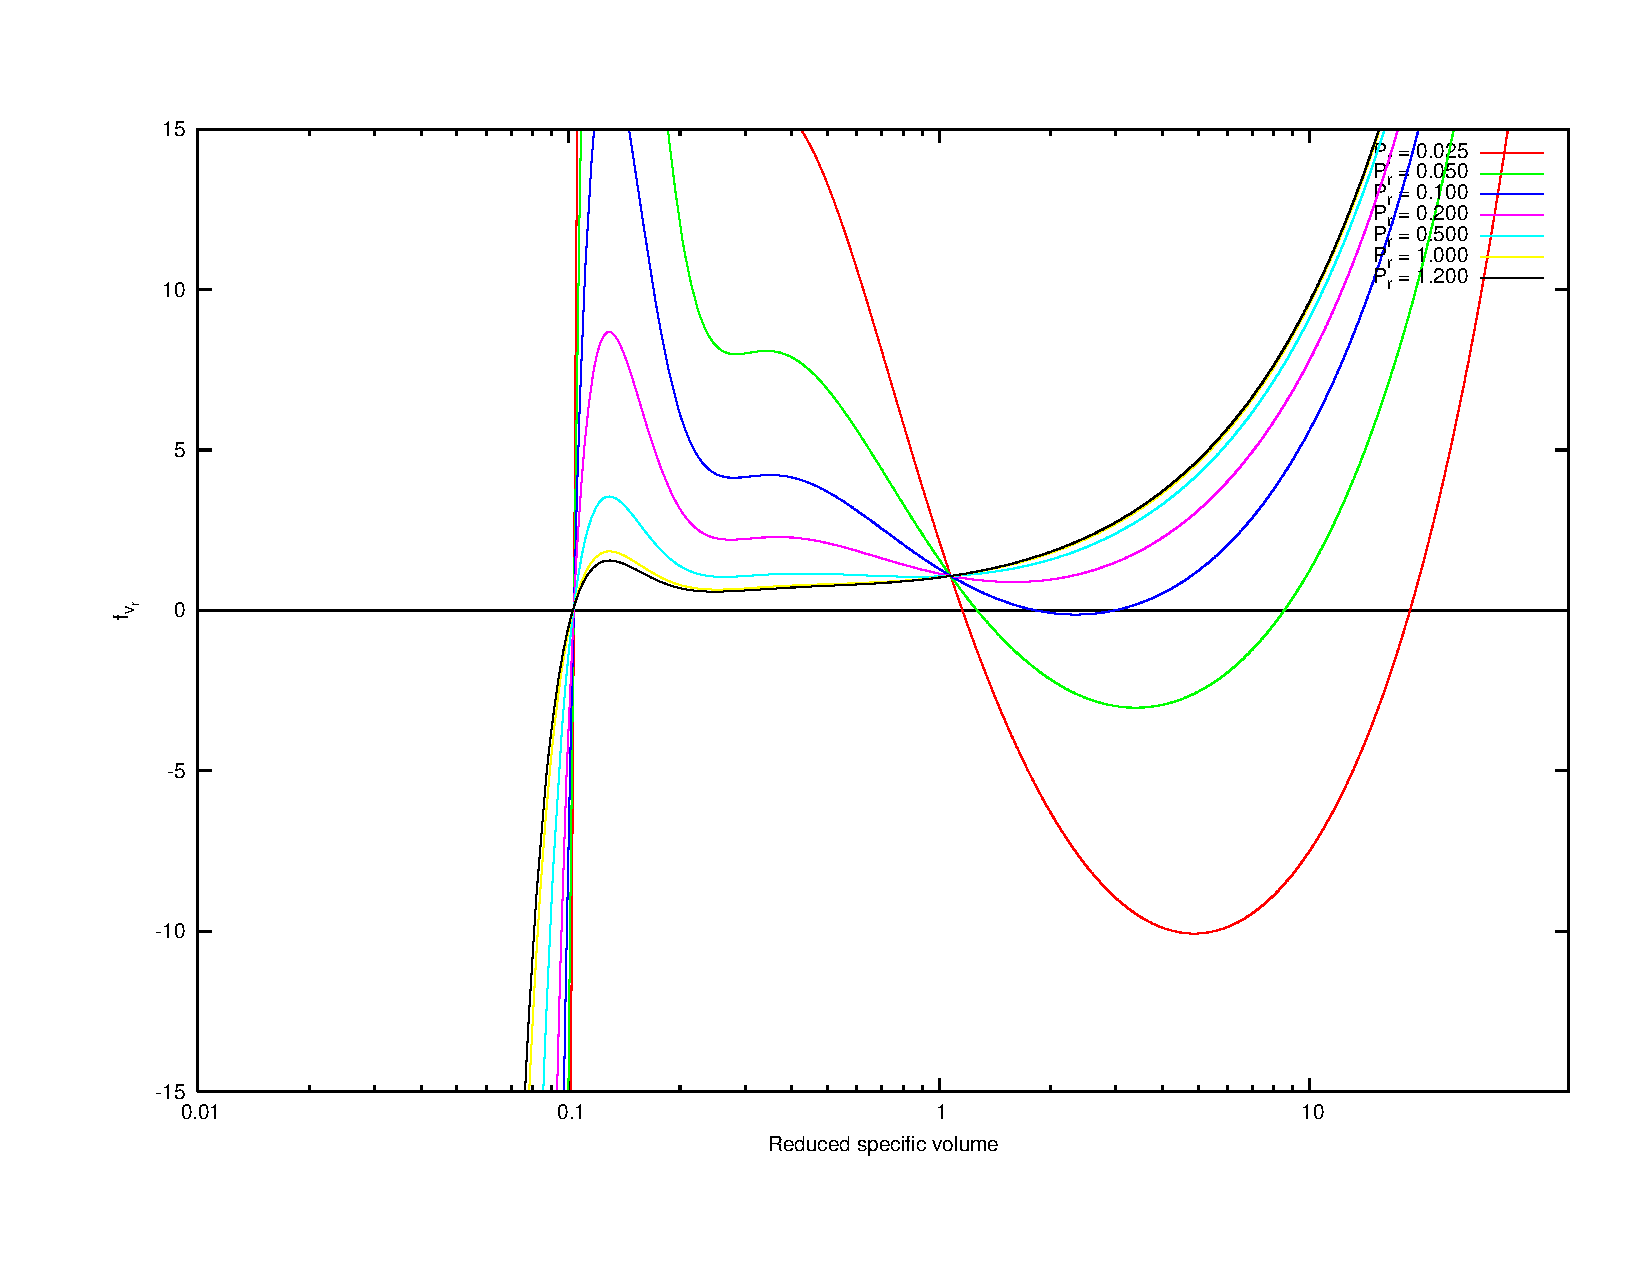
\includegraphics[trim = 1.5cm 2cm 0 1cm, clip = true, width=14cm]{05Tc_3}
  \caption{$f$ as a function of reduced specific volume, for $T_r = 0.500$. Reduced pressure is varied from 0.025 to 1.200. Fluid is a simple fluid mixture with 0.5 moles of CO$_2$ and 0.5 moles of methane.}
  \label{fig:0.5Tc}
\end{figure}

\begin{figure}[h]
  \centering
  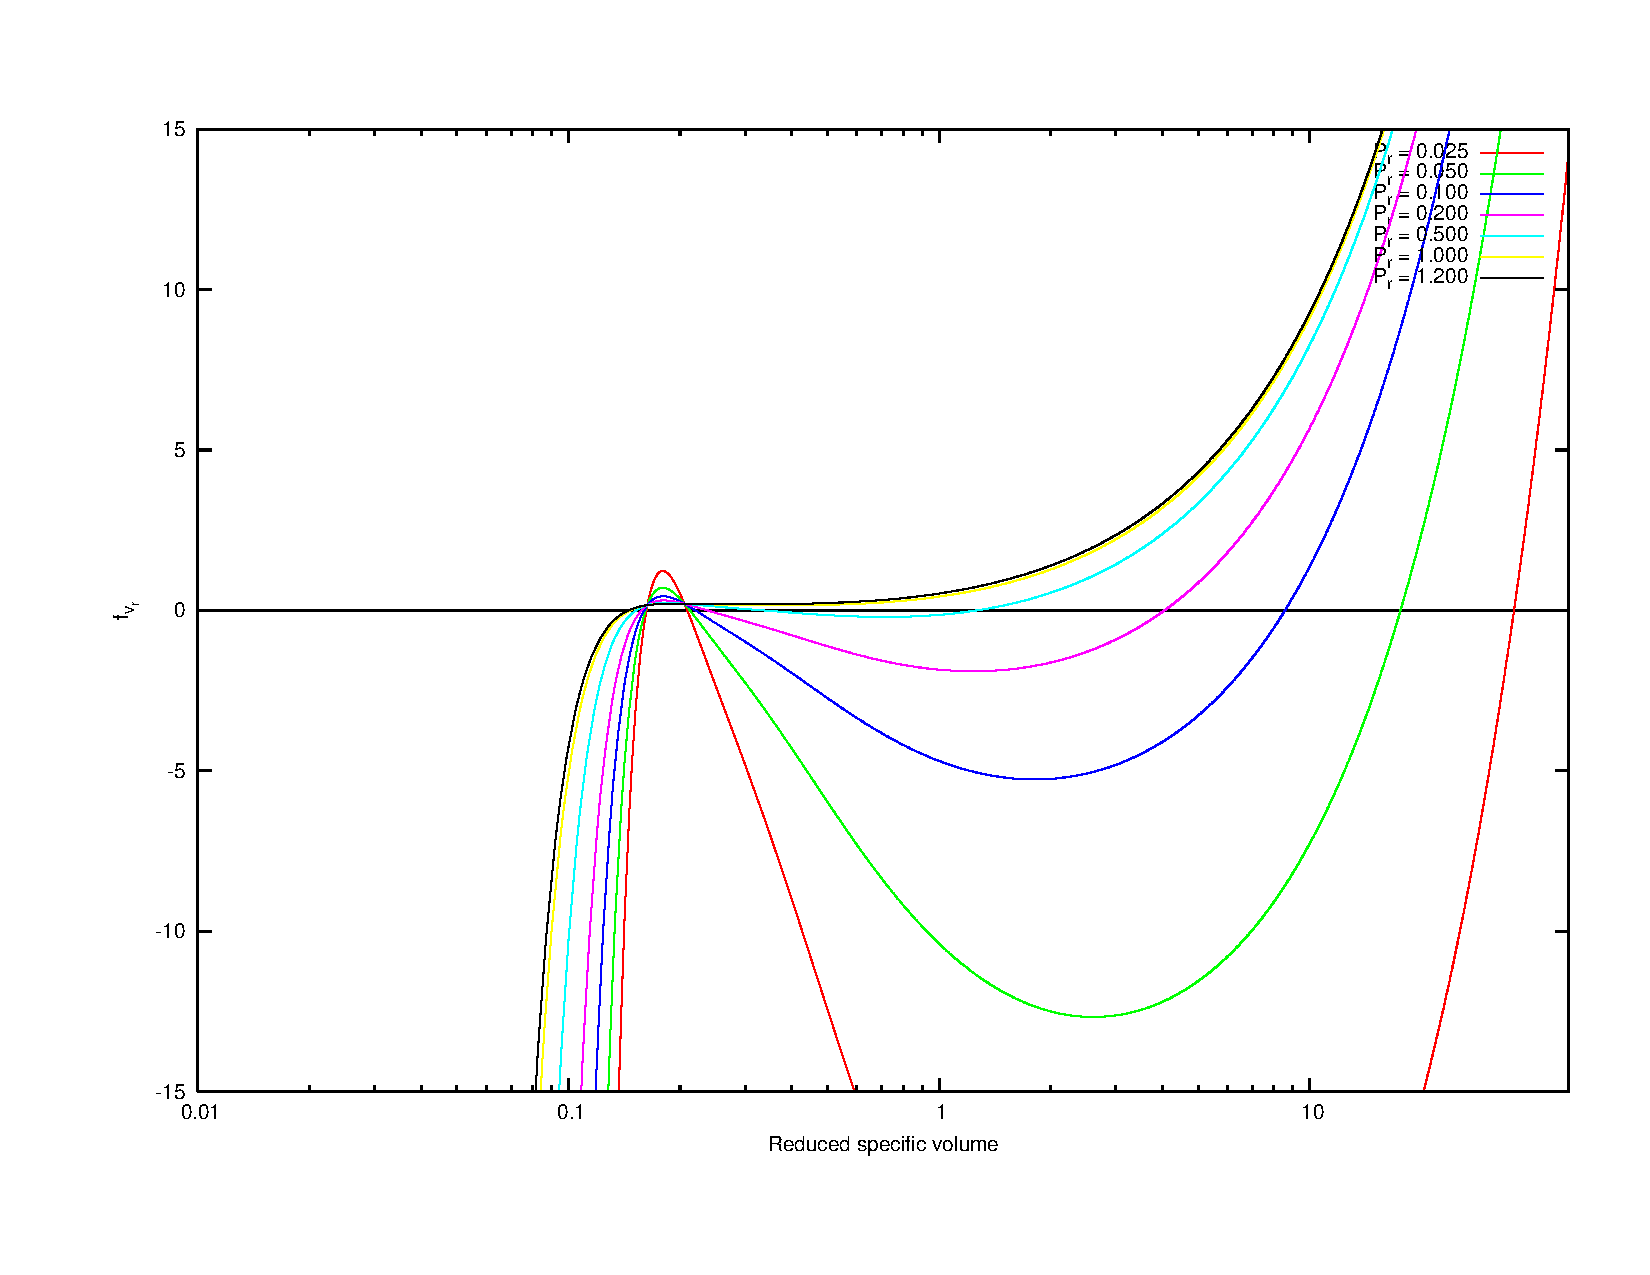
\includegraphics[trim = 1.5cm 2cm 0 1cm, clip = true, width=14cm]{09Tc_3}
  \caption{$f$ as a function of reduced specific volume, for $T_r = 0.900$. Reduced pressure is varied from 0.025 to 1.200. Fluid is a simple fluid mixture with 0.5 moles of CO$_2$ and 0.5 moles of methane.}
  \label{fig:0.9Tc}
\end{figure}

\begin{figure}[h]
  \centering
  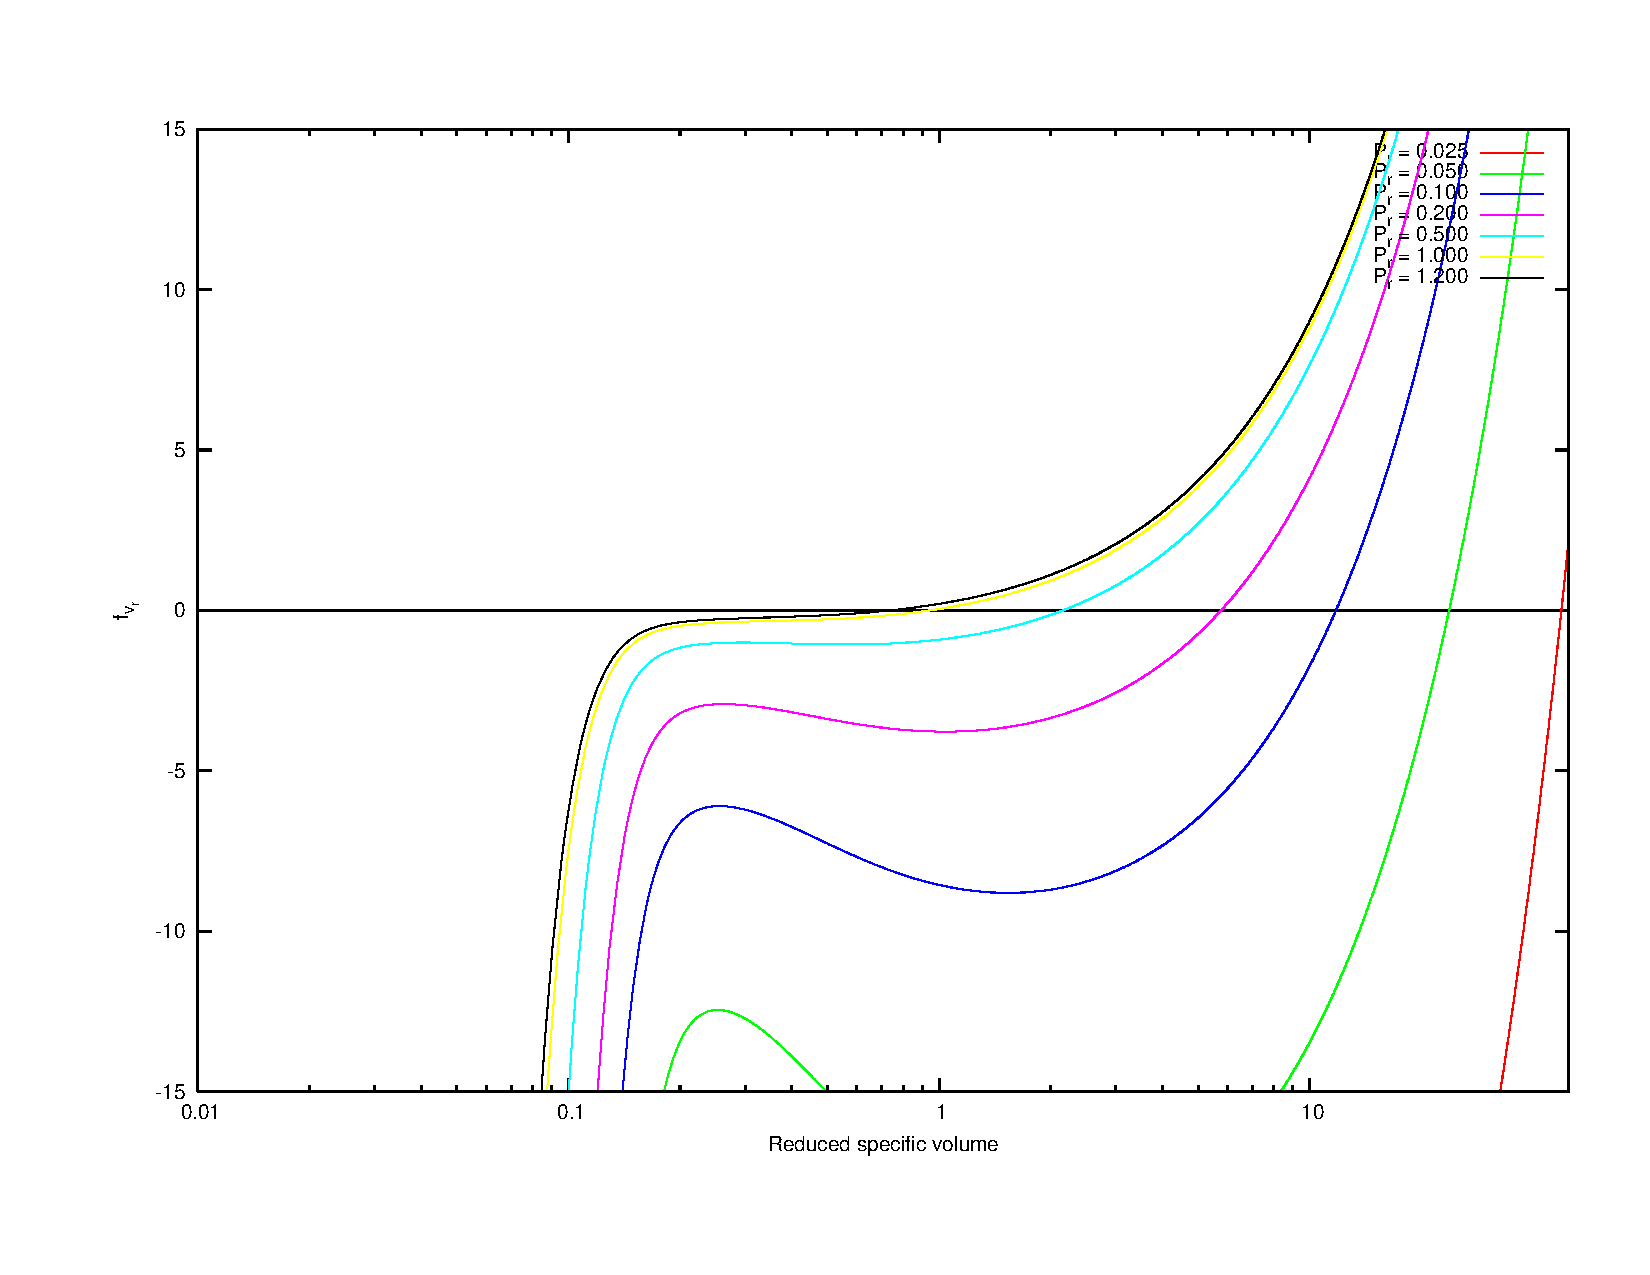
\includegraphics[trim = 1.5cm 2cm 0 1cm, clip = true, width=14cm]{12Tc_3}
  \caption{$f$ as a function of reduced specific volume, for $T_r = 1.200$. Reduced pressure is varied from 0.025 to 1.200. Fluid is a simple fluid mixture with 0.5 moles of CO$_2$ and 0.5 moles of methane.}
  \label{fig:1.2Tc}
\end{figure}

The main problem in solving the equation for $f(v_r) = 0$ is finding a good initial value for the reduced specific volume. Since Equation \reff{eq:fv} is identical whether it is solved for a fluid in liquid or gas phase, but the real value for the volume obviously is not the same, a good initial guess must take into account what phase the solution is intended for. In addition to this, constrains must be found, that ensures that the numerical solution is not wander off into another phase than that intended. 

In calculating this initial value, an initial value finder made by Anders Austegard, in the previous implementation of the Lee-Kesler method, is used. This routine takes reduced temperature, reduced pressure, phase and an integer that separates simple fluid calculations from reference fluid calculations, as input. It returns an initial value for the reduced specific volume, and minimal and maximal bound for it. This routine does however not take into account whether the fluid physically may exists in both liquid and gas phase at the given reduced temperature and pressure.

By studying once more Figures \ref{fig:0.5Tc} and \ref{fig:0.9Tc} it is clear that, for each of the reduced temperatures, several roots exist for a reduced pressure below a certain threshold pressure. Physically, what happens at when increasing the pressure past this threshold, is that the the fluid goes from a state where both liquid and gas phases are allowed, to a state where only liquid phase is allowed.

\begin{figure}
	\centering
	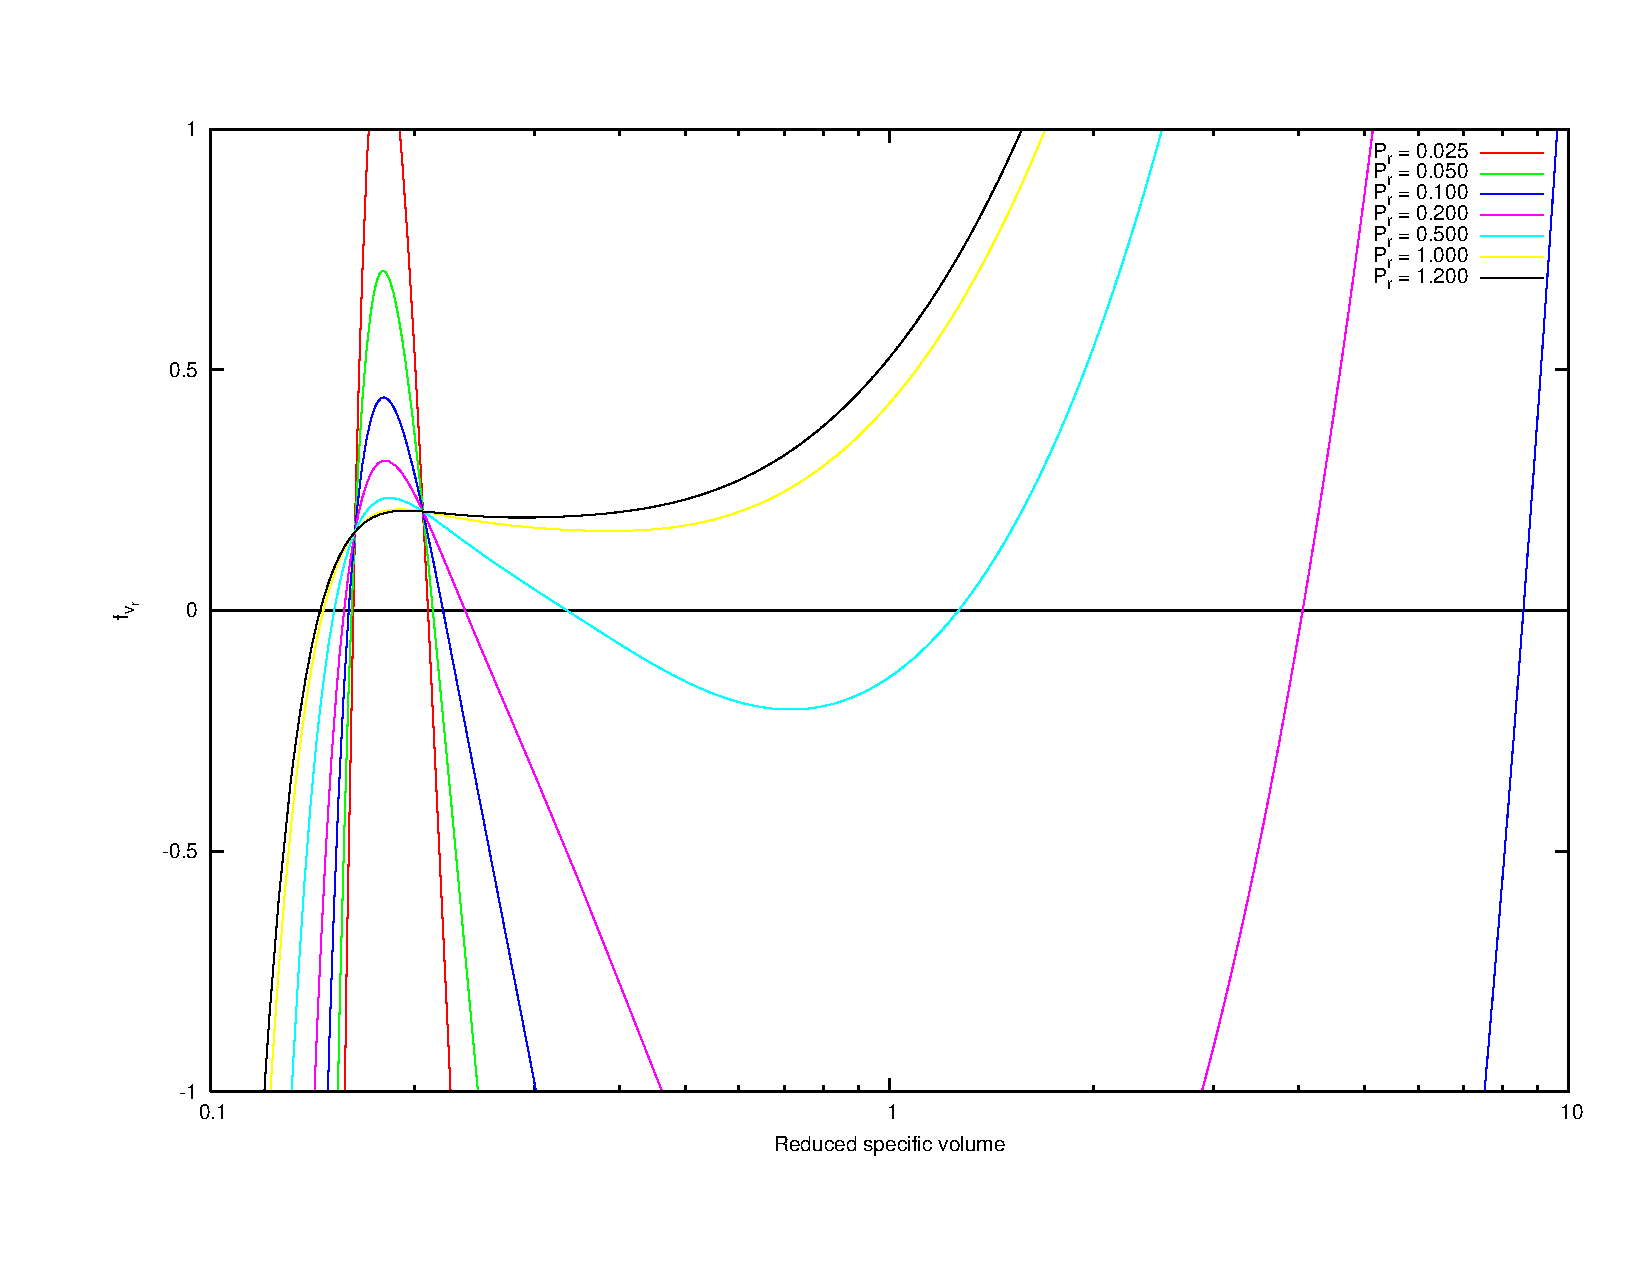
\includegraphics[trim = 1.5cm 2cm 0 1cm, clip = true, width=14cm]{09TcZoom}
	\caption{$f$ as a function of reduced specific volume, for $T_r = 0.900$. Reduced pressure is varied from 0.025 to 1.200. Fluid is a simple fluid mixture with 0.5 moles of CO$_2$ and 0.5 moles of methane. View is zoomed compared to Figure \ref{fig:0.9Tc}.}
	\label{fig:0.9TcZoom}
\end{figure}

Consider Figure \ref{fig:0.9TcZoom}. This is a zoomed view of the calculations plotted in Figure \ref{fig:0.9Tc}. Studying this figure brings attention to a major challenge in calculation the reduced specific volume. The lower root for the pressure curves in Figure \ref{fig:0.9TcZoom} is the physical solution of the reduced volume in liquid phase, while the highest valued root is the physical solution of the reduced volume in gas phase (for the reduced pressure values that yield more than one root). In between these there is a third root. This is \textit{not} a physical state for the fluid, and must not be interpreted as one. The initial value solver takes this into account when setting up the allowed interval for $v_r$, and the half step method is used to ensure that $v_r$ is within its limits during the iterations in the Newton-Raphson method.

There of course also exists states for the fluid where the only valid phase is either the liquid phase or the gas phase. The curves with reduced pressure $P_r \geq 0.200$ in Figure \ref{fig:0.5Tc} are example of states where the mixture only exists in liquid phase. In contrast, the curves with $P_r \leq 0.500$ in Figure \ref{fig:1.2Tc} represent states where only the gas phase is the correct physical solutions. The two curves where $P_r \geq 1.000$ in the same figure represent supercritical states, where no distinct liquid or gas phase exist. 

One of the input parameters to the Lee-Kesler module is the phase of the fluid mixture. Problems will arise for states where this user defined phase does not exist. And even if it exists, it is not certain that the phase is the equilibrium solution for the system. To cope with the first of these problems, the numerical calculation subroutine returns a boolean variable \textit{correctPhase}, that is true if there exists a solution for the the phase chosen by the user, and false if not. The main subroutine in the module checks this variable, and if it is false, changes phase (with a prompt to the user) before calculating the reduced specific volume once more. 

At this time there is not implemented any equilibrium solution checker in the module, that can return the equilibrium properties, for states where several phases exists, if specified by the user. This can however be done quite straightforwardly: By using the fact that the Gibbs free energy has a minima at an equilibrium point, the equilibrium can be found by calculating this thermodynamic property for both available solutions for $v_r$, and choosing the smallest one. Calculation of Gibbs free energy can be done from the Helmholtz function $F$, and therefore does not require any major modifications in the program.

\begin{figure}
	\centering
	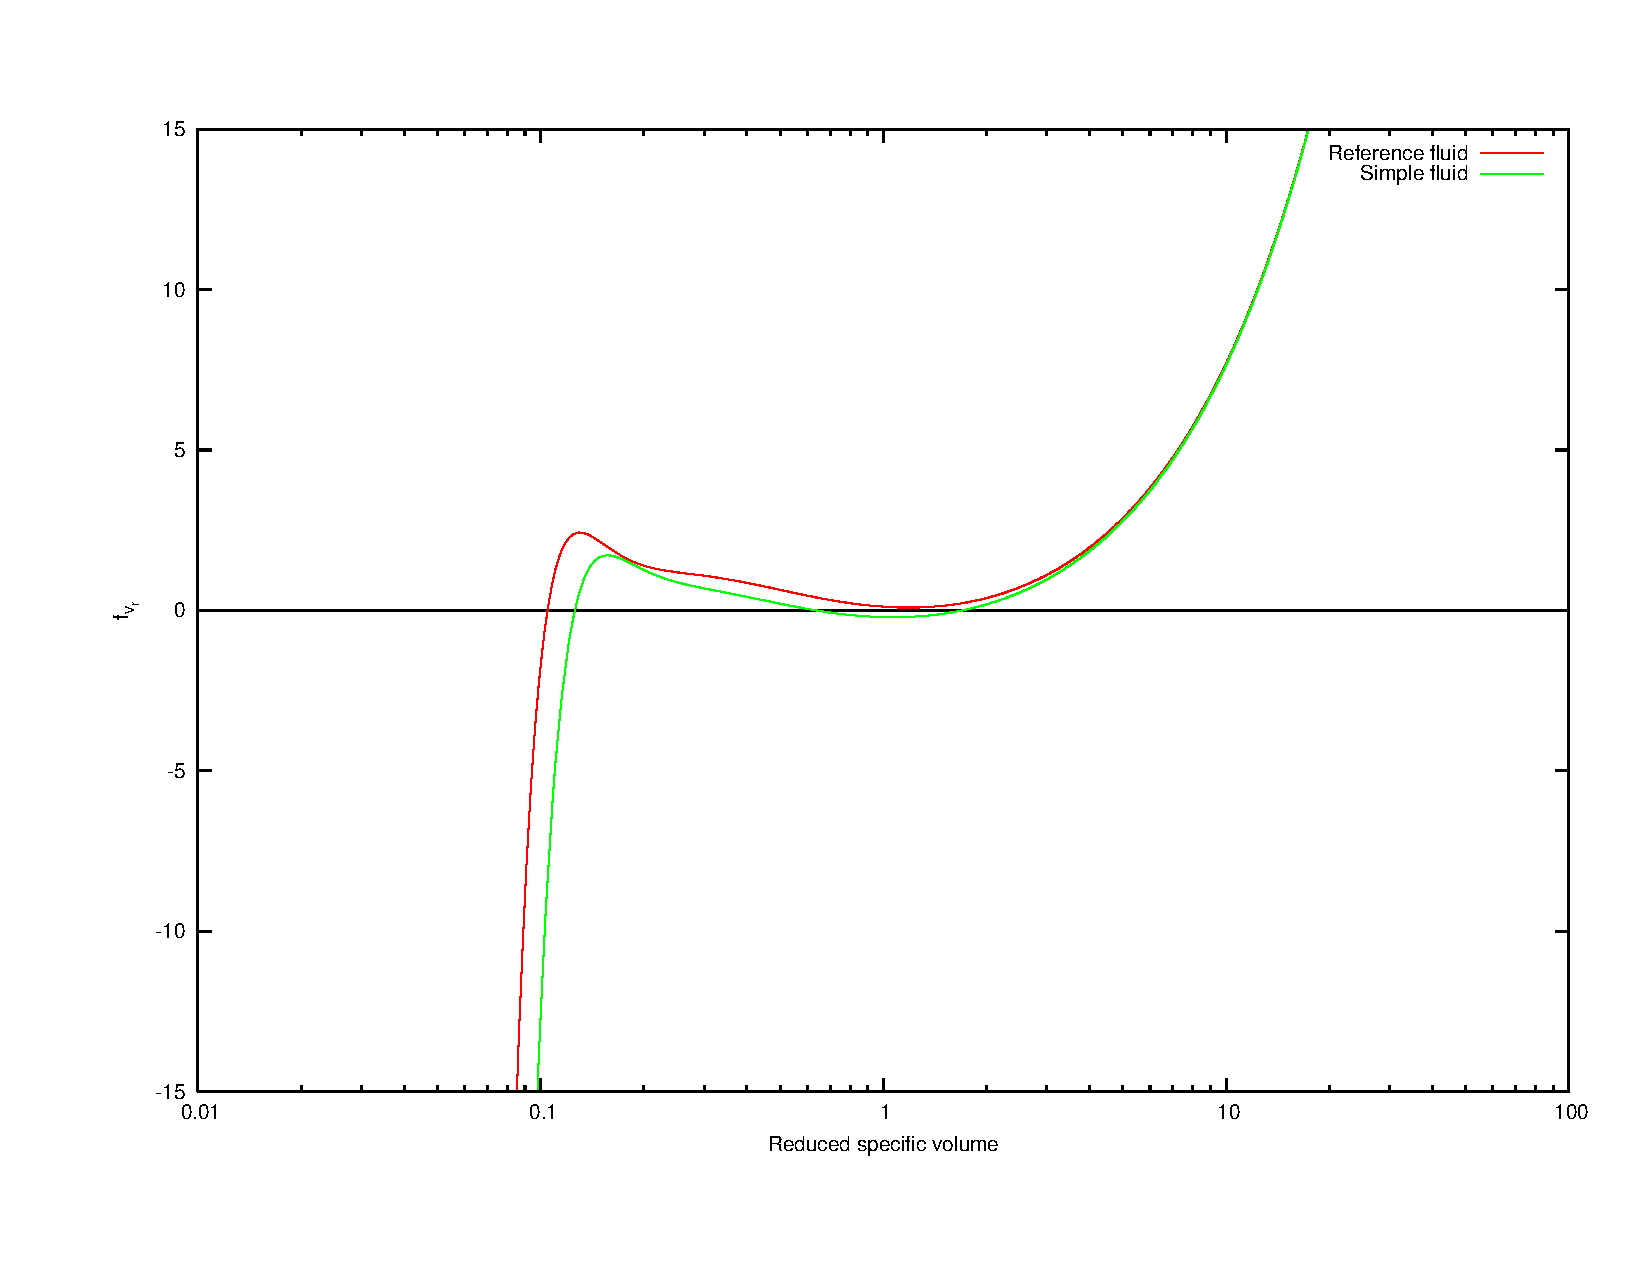
\includegraphics[trim = 1.5cm 2cm 0 1cm, clip = true, width=14cm]{075Tc_SR}
	\caption{$f$ as a function of reduced specific volume, for $T_r = 0.750$ and $P_r = 0.300$. The fluid is a mixture with 0.5 moles of CO$_2$ and 0.5 moles of methane. Calculations for a simple fluid and a reference fluid are plotted.}
	\label{fig:vrSimpRef}
\end{figure}

Consider Figure \ref{fig:vrSimpRef}. This is a plot of Equation \reff{eq:fv} for a simple fluid and a reference fluid, with $T_r = 0.750$ and $P_r = 0.300$, for the same fluid mixture as before. The figure illustrates another pitfall, when calculation the reduced specific volume of the mixture: for some relations between reduced temperature and pressure, a only single phase solution exists for the reference fluid, but two solutions exist for the simple fluid, or vice versa. If $v_r$ is calculated for gas for the simple fluid, but switched to liquid for the reference fluid, the aggregated results for departure entropy, enthalpy etc. will be dead wrong. To avoid this, when performing the check of the variable \textit{correctPhase}, if it is false for either the simple or reference fluid (or both), the phase is changed, and both simple volume calculations are done over, with the new phase defined.

\subsection{Compiling and executing the code}
During the implementation, compilation of the code has been done by a \textit{make run} command in the \textit{command prompt} on a Windows 7 machine. The makefile called upon is found in the mingw32 folder in ThermoPack, and has been modified to fit the needs of the Lee-Kesler module, by Morten Hammer. A main file initializes ThermoPack, and build a vector with the critical properties of the components specified in the same file. Temperature and pressure, as well as phase, are also specified here, and a call is made upon the \textit{mainLeeKesler}-subroutine. The approach is rather primitive, but is intended to make it easy to fit the module into ThermoPack, so that it can be called upon there, as any other equation of state. 

\section{Results and discussion}
In this section, the results presented are consistency tests according to the identities in Subsection \ref{subsec:consistCheck}, and the calculated values for the thermodynamic properties of interest. These properties are compressibility factor, departure entropy, departure enthalpy and component fugacity coefficients, given by equations \reff{def:z}, \reff{def:S^R(T,V,n)} and \reff{def:S^R(T,V,n)}, \reff{def:H^R(T,P,n)}, and \reff{def:lnphi(T,P,n)}. The first three of these are compared to the tabulated values in \cite{LK}, but since the component fugacity coefficients are not presented here, they are compared with values calculated by a cubic equations of state.

\subsection{Consistency tests}
Two results are presented for the consistency test identities. One is magnitude of the deviation, where the identities given by Equations \reff{test:1} - \reff{test:8} are all rewritten to be zero, hence the deviation is the deviation from the zero value. The smaller deviation the better. The second result is the relative deviation. This is given for all tests except Equation \reff{test:6}, that is, all test that can written in the form, $I_1 = I_2$, where $I_1$ and $I_2$ together make up any of the eight identities. The Relative deviation is then given by:
\begin{equation}
\frac{\Delta I}{I} = \frac{I_1 - I_2}{I_1}
\end{equation}

The tests are performed for arbitrary values of reduced temperature, reduced pressure and composition, but it is ensured that both sub- an supercritical values are tested. The phase is set to gas for all calculations, but automatically changed to liquid, where gas phase is not an allowed solution. Calculations are done separately for simple fluid and reference fluid; only the largest deviation is given in the tables. For identities where there is an index that is summed over, this index is set to one.

\begin{table}[h!]
  \centering
    \caption{Test of the partial derivatives of the Helmholtz function.}
    \label{tab:testHelmholtz}
    \begin{tabular}{c c c c c c c}
      \hline
      Test 			& $T_r$ & $P_r$ & CO$_2$	& Methane	& Deviation 		& Relative deviation \\
      equation		&		&		& \# moles	& \# moles	& $\Delta I$		& $\frac{\Delta I}{I}$\\
      \hline
      \reff{test:1}	& 0.100	& 0.050	& 0.95		&0.50		& $10^{-13}$ 	& $10^{-14}$	\\
      				& 0.200	& 0.050	& 0.95		&0.10		& $10^{-14}$	& $10^{-16}$	\\
      				& 0.900	& 0.800	& 0.60		&0.50		& $10^{-16}$	& $10^{-16}$	\\
      				& 0.900	& 1.200	& 0.60		&0.10		& $10^{-16}$	& $10^{-16}$	\\
      				& 1.150	& 1.250	& 0.10		&0.50		& $10^{-17}$	& $10^{-16}$	\\
      \reff{test:2}	& 0.100	& 0.050	& 0.95		&0.50		& $10^{-11}$	& $10^{-16}$	\\
      				& 0.200	& 0.050	& 0.95		&0.10		& $10^{-14}$	& $10^{-16}$	\\
      				& 0.900	& 0.800	& 0.60		&0.50		& $10^{-15}$	& $10^{-16}$	\\
      				& 0.900	& 1.200	& 0.60		&0.10		& $10^{-15}$	& $10^{-16}$	\\
      				& 1.150	& 1.250	& 0.10		&0.50		& $10^{-15}$	& $10^{-16}$	\\
      \reff{test:3}	& 0.100	& 0.050	& 0.95		&0.50		& $10^{-7}$		& $10^{-16}$	\\
      				& 0.200	& 0.050	& 0.95		&0.10		& $10^{-8}$		& $10^{-16}$	\\
      				& 0.900	& 0.800	& 0.60		&0.50		& $10^{-11}$	& $10^{-16}$	\\
      				& 0.900	& 1.200	& 0.60		&0.10		& $10^{-11}$	& $10^{-16}$	\\
      				& 1.150	& 1.250	& 0.10		&0.50		& $10^{-13}$	& $10^{-16}$	\\
      \hline
    \end{tabular}
\end{table}

\begin{table}[h!]
  \centering
    \caption{Test results for the fugacity coefficient identities.}
    \label{tab:testFugacity}
    \begin{tabular}{c c c c c c c}
      \hline
      Test 			& $T_r$ & $P_r$ & CO$_2$	& Methane	& Deviation		& Relative deviation\\
      equation		&		&		& \# moles	& \# moles	& $\Delta I$		& $\frac{\Delta I}{I}$\\
      \hline
      \reff{test:4}	& 0.100	& 0.050	& 0.95		&0.50		& $10^{-11}$	& $10^{-13}$	\\
      				& 0.200	& 0.050	& 0.95		&0.10		& $10^{-14}$	& $10^{-15}$	\\
      				& 0.900	& 0.800	& 0.60		&0.50		& $10^{-16}$	& $10^{-16}$	\\	
      				& 0.900	& 1.200	& 0.60		&0.10		& $10^{-15}$	& $10^{-16}$	\\
      				& 1.150	& 1.250	& 0.10		&0.50		& $10^{-16}$	& $10^{-16}$	\\
      \reff{test:5}	& 0.100	& 0.050	& 0.95		&0.50		& $10^{-12}$	& $10^{-13}$	\\
      				& 0.200	& 0.050	& 0.95		&0.10		& $10^{-14}$	& $10^{-14}$	\\
      				& 0.900	& 0.800	& 0.60		&0.50		& $10^{-16}$	& $10^{-16}$	\\
      				& 0.900	& 1.200	& 0.60		&0.10		& $10^{-16}$	& $10^{-15}$	\\
      				& 1.150	& 1.250	& 0.10		&0.50		& $10^{-17}$	& $10^{-16}$	\\
      \reff{test:6}	& 0.100	& 0.050	& 0.95		&0.50		& $10^{-11}$	& - 	\\
      				& 0.200	& 0.050	& 0.95		&0.10		& $10^{-14}$	& - 	\\
      				& 0.900	& 0.800	& 0.60		&0.50		& $10^{-13}$	& - 	\\
      				& 0.900	& 1.200	& 0.60		&0.10		& $10^{-15}$	& -		\\
      				& 1.150	& 1.250	& 0.10		&0.50		& $10^{-16}$	& - 	\\
      \reff{test:7}	& 0.100	& 0.050	& 0.95		&0.50		& $10^{-22}$	&  $10^{-17}$	\\
      				& 0.200	& 0.050	& 0.95		&0.10		& $10^{-22}$	&  $10^{-17}$ 	\\
      				& 0.900	& 0.800	& 0.60		&0.50		& $10^{-23}$	&  $10^{-16}$	\\
      				& 0.900	& 1.200	& 0.60		&0.10		& $10^{-24}$	&  $10^{-17}$	\\
      				& 1.150	& 1.250	& 0.10		&0.50		& $10^{-23}$	&  $10^{-15}$	\\
      \reff{test:8}	& 0.100	& 0.050	& 0.95		&0.50		& $10^{-14}$	&  $10^{-16}$	\\
      				& 0.200	& 0.050	& 0.95		&0.10		& $10^{-16}$	&  $10^{-16}$	\\
      				& 0.900	& 0.800	& 0.60		&0.50		& $10^{-17}$	&  $10^{-16}$	\\
      				& 0.900	& 1.200	& 0.60		&0.10		& $10^{-18}$	&  $10^{-16}$	\\
      				& 1.150	& 1.250	& 0.10		&0.50		& $10^{-18}$	&  $10^{-16}$	\\
      \hline
    \end{tabular}
\end{table}

The results for the identity consistency test presented in Table \ref{tab:testHelmholtz} and \ref{tab:testFugacity} are very good, and indicate that all the analytical derivatives that are part of these tests are analytically correct. One might expect that the deviation should be exactly zero, since this is the analytical result. The $10^{-16}$ magnitude of the relative deviation practically equals zero deviation in the analytical result, since this deviation is due to the number of digits in the $real$ data type used in the FORTRAN 90 implementation. If all the digits in the real are equal, subtraction one from another does not necessarily give zero as a result. It rather gives the result of subtraction by the random digits \textit{behind} the stored digits in the reals, which start at one magnitude smaller than the smallest valid decimal point.

In addition to the consistency tests results presented here, all analytical derivative functions Tables \ref{tab:functionsF} and \ref{tab:functionsTherm} in Appendix \ref{app:subFunc}, have been compared to their numerical derivatives, using by Equations \reff{eq:numDir1} - \reff{eq:numDir5}. Hence, all analytical derivatives should be correct.

\subsection{Direct comparison to tabulated values}
\label{subsec:dircomp}
The original article by Lee and Kesler \cite{LK} include a large set of data, which give calculated values for the compressibility factor, departure entropy, departure enthalpy, mixture fugacity coefficient and departure heat capacity. The first of these three match thermodynamic properties calculated in this implementation of the method, and serve as a good set of data for comparison with calculated values. The data for the compressibility factor is given as $z^{(0)}$ and $z^{(1)} = (z^{(r)} - z^{(0)})/\omega^{(r)}$, where the superscripts are consistent with the notation in this report. Similarly the negatives of $S_{dep}^{(0)}$, $S_{dep}^{(1)}$, $H_{dep}^{(0)}$ and $H_{dep}^{(1)}$ can be found in the tables in the article. 

All tabulated values are given for reduced temperature and reduced pressure, hence they should be valid for any fluid mixture. The fluid mixture used here is a 50-50 mix of CO$_2$ and methane. This gives critical mixing values: $T_{cM} \simeq 237.8$ K, $P_{cM} \simeq 57.9$ bar. Only a few selected reduced temperatures plotted, to avoid that the plots getting too messy. The pressure in the calculated results, and in the tabulated values, is varied from $P_r = 0.010$ to $P_r = 10.000$.

\subsubsection*{Compressibility}
\begin{figure}
	\centering
	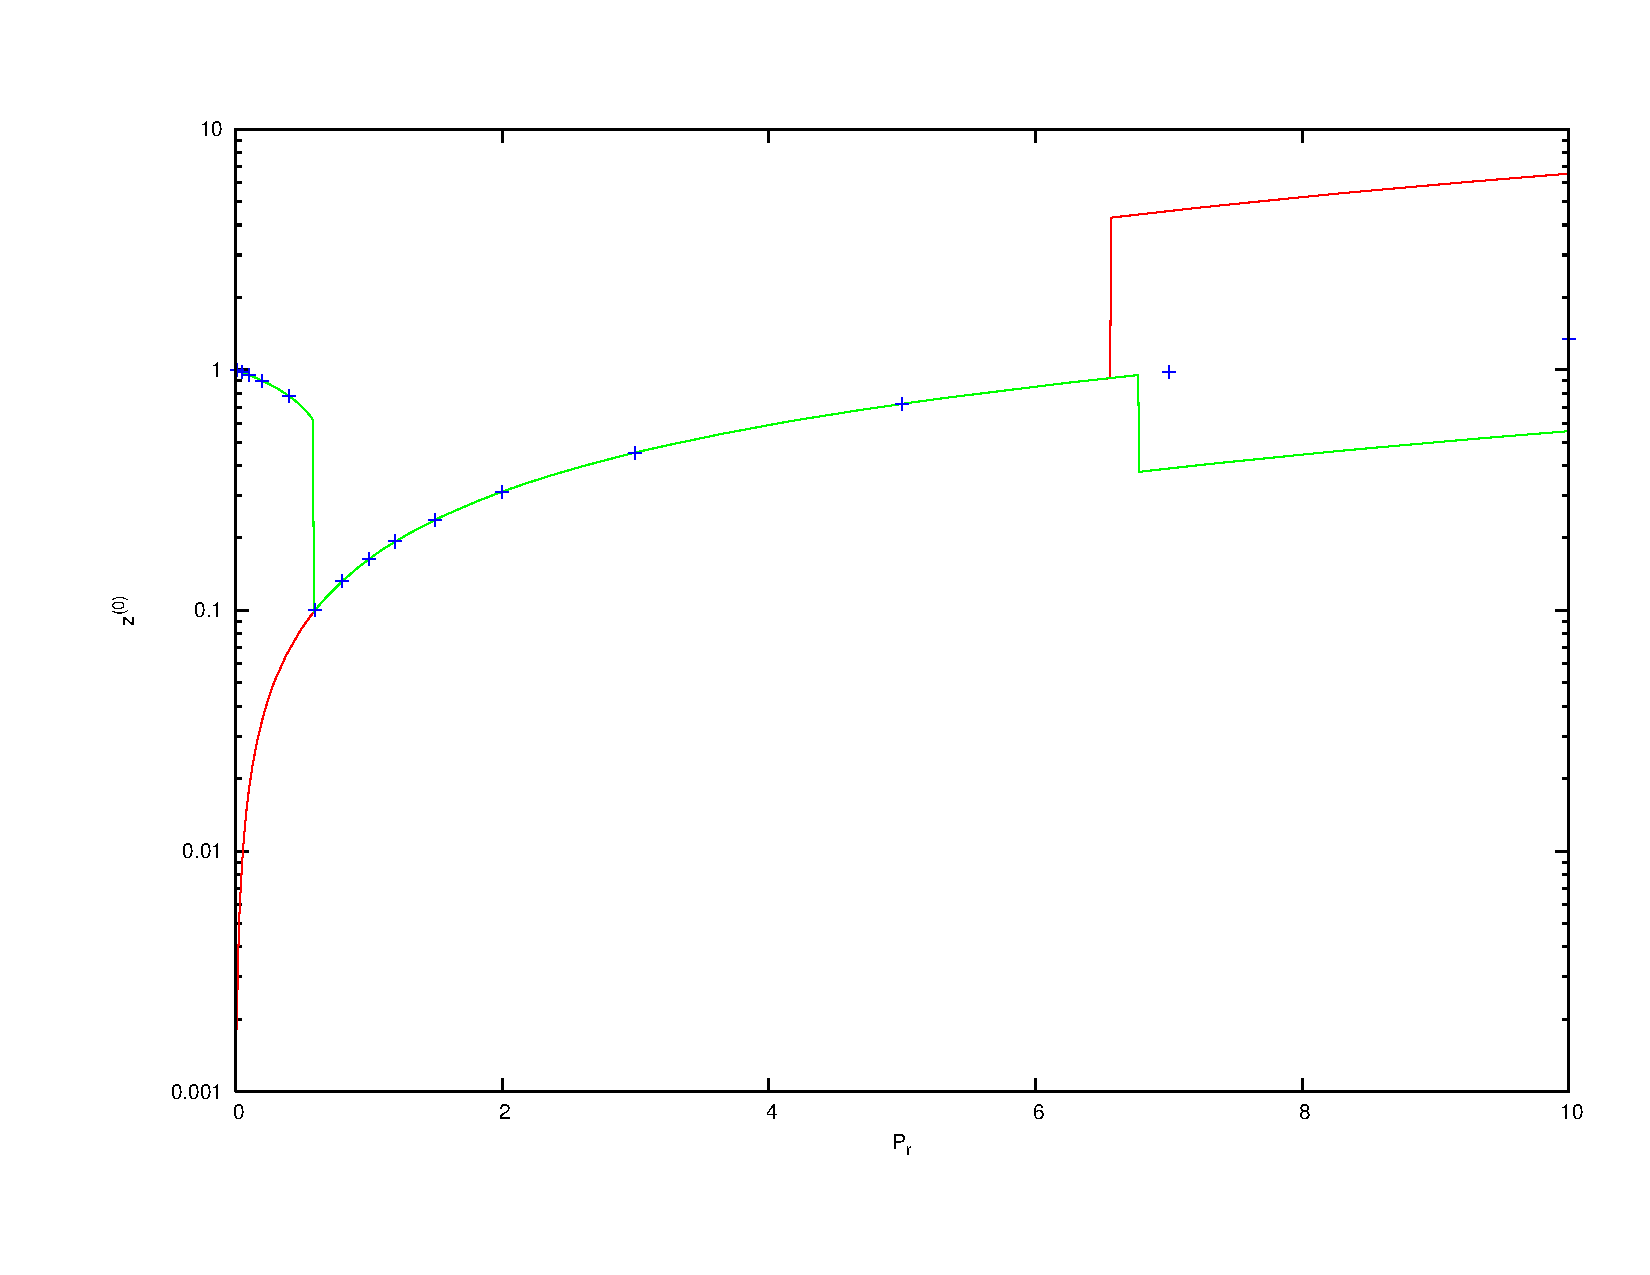
\includegraphics[trim = 1.5cm 2cm 0 1cm, clip = true, width=14cm]{z0Tc090}
	\caption{$z^{(0)}$ as a function of reduced pressure, for $T_r = 0.900$. Line plots show computational results with phase set to liquid (red) and gas (green), respectively. Data points show tabulated values from Table 5 in \cite{LK}}
	\label{fig:z0Tc090}
\end{figure}

Consider Figure \ref{fig:z0Tc090}. For low pressures ($P_r < 0.600$) both the liquid phase and the gas phase exist. It is assumed that only one of these is an equilibrium solution, and as seen in the figure, the tabulated data points give an exact match with the computational results for phase set to gas. For $P \geq 0.600$ only the liquid phase is a physically acceptable solution. Therefore, the phase is forced to liquid, for both computational runs. The results match exactly with the tabulated results, until $P_r > 5.000$. There is a large, seemingly discontinuous deviation for both the gas calculations and the liquid calculations from $P_r \approx 6.5$ and beyond. This is the area where no numerical solution for the reduced specific volume is found by the method implemented here.

The results plotted in Figure \ref{fig:z0Tc090} represent typical behaviour of the simple fluid compressibility factor, calculated by this implementation. The area of deviation, caused by the absence of a good result for $v_r$, is larger (it occurs for a lower pressure) for a smaller reduced temperature, and smaller for a larger reduced temperature. During the implementation and testing of this module, few calculations have been done for reduced pressures larger than 1.5. However, to further improve the calculations, the shape of $f$ in Equation \reff{eq:fv} should be studied for large pressures, and an improvement made to the numerical solver, to cope with these pressures. Ideally, behaviour as seen for $P_r > 6.5$ will then be eliminated from the program.

The pressure interval where both gas and liquid are valid solution varies with different reduced temperature. For some temperatures, only a single phase is a valid solutions, for all pressures. However, if this is not the case, as seen in Figure \ref{fig:z0Tc090} for $P_r < 0.600$, this interval may give rise to errors when using the program: If the user is only after the equilibrium solution, the wrong result will be calculated if the non-equilibrium phase is specified, as mentioned in \ref{subsec:v_r}.

\begin{figure}
	\centering
	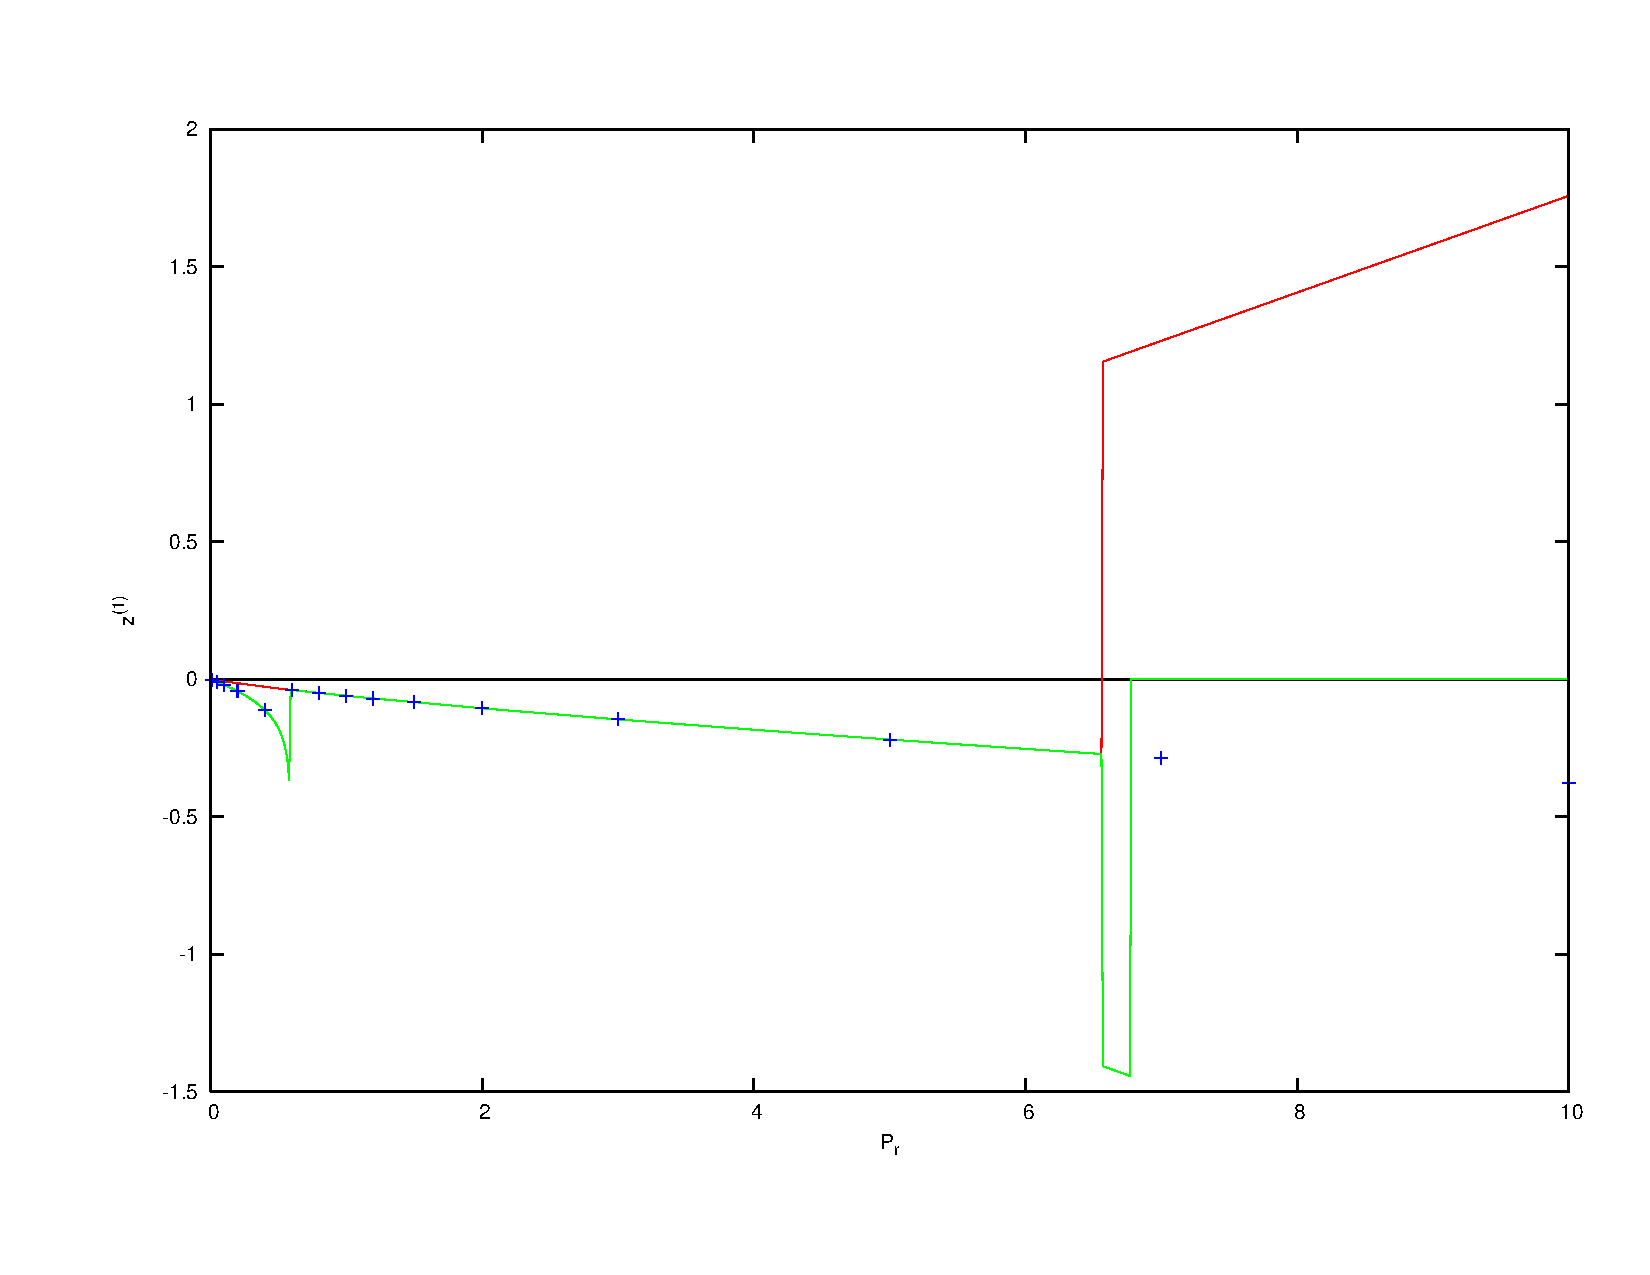
\includegraphics[trim = 1.5cm 2cm 0 1cm, clip = true, width=14cm]{z1Tc090}
	\caption{$z^{(1)}$ as a function of reduced pressure, for $T_r = 0.900$. Line plots show computational results with phase set to liquid (red) and gas (green), respectively. Data points show tabulated values from Table 6 in \cite{LK}}
	\label{fig:z1Tc090}
\end{figure}

The results for $z^{(1)}$ presented in Figure \ref{fig:z1Tc090} are very similar to the ones in Figure \ref{fig:z0Tc090}. Although the numerical values are quite different, the troublesome regions occur at the same pressures. This is expected, as it is the reduced specific volume calculations that give rise to these phenomena. 

Over all, the results for the compressibility, $z^{(0)}$ and $z^{(1)}$ are good, for a large pressure interval, for the reduced temperature studied here. This is also true for a quite large interval of reduced temperatures. 

\subsubsection*{Departure Entropy}
\begin{figure}
	\centering
	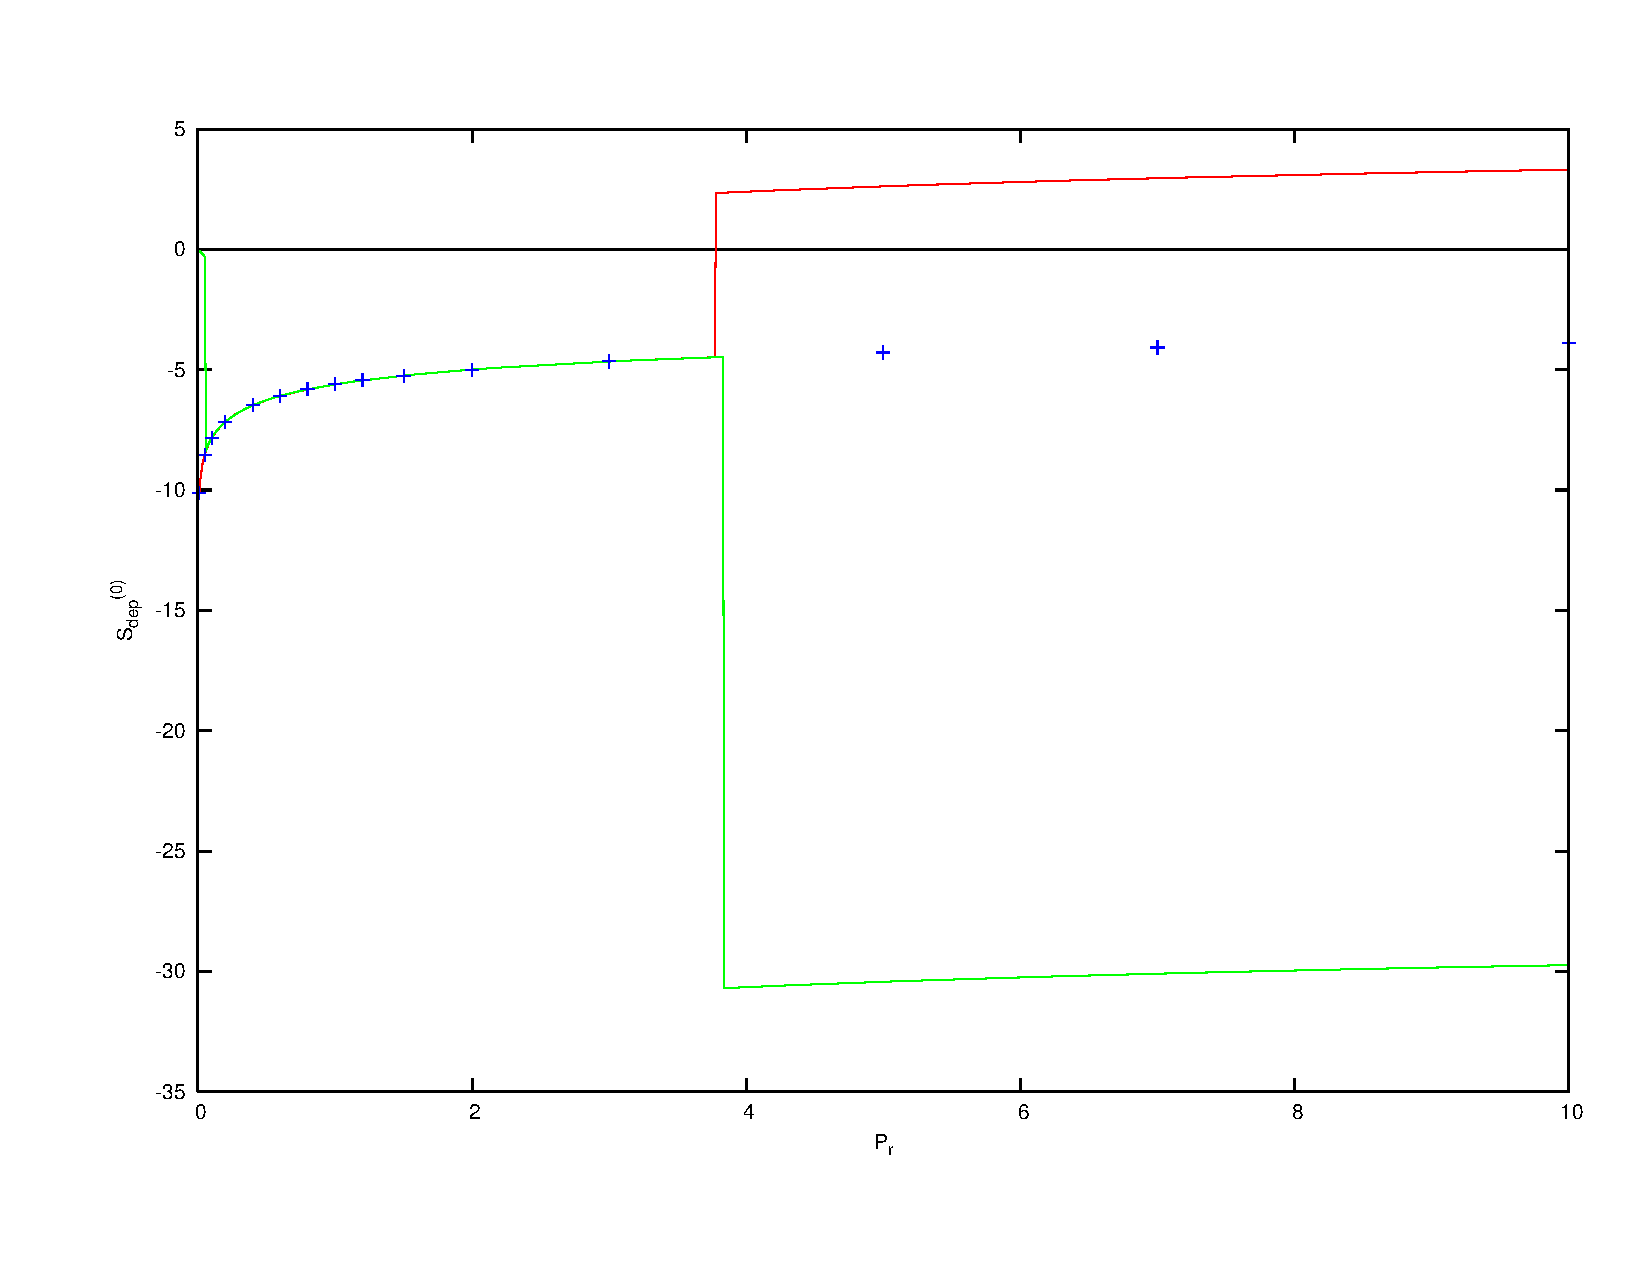
\includegraphics[trim = 1.5cm 2cm 0 1cm, clip = true, width=14cm]{Sdep0Tc050}
	\caption{$S_{dep}^{(1)}$ as a function of reduced pressure, for $T_r = 0.500$. Line plots show computational results with phase set to liquid (red) and gas (green), respectively. Data points show the negatives of tabulated values from Table 9 in \cite{LK}}
	\label{fig:Sdep0Tc050}
\end{figure}

\begin{figure}
	\centering
	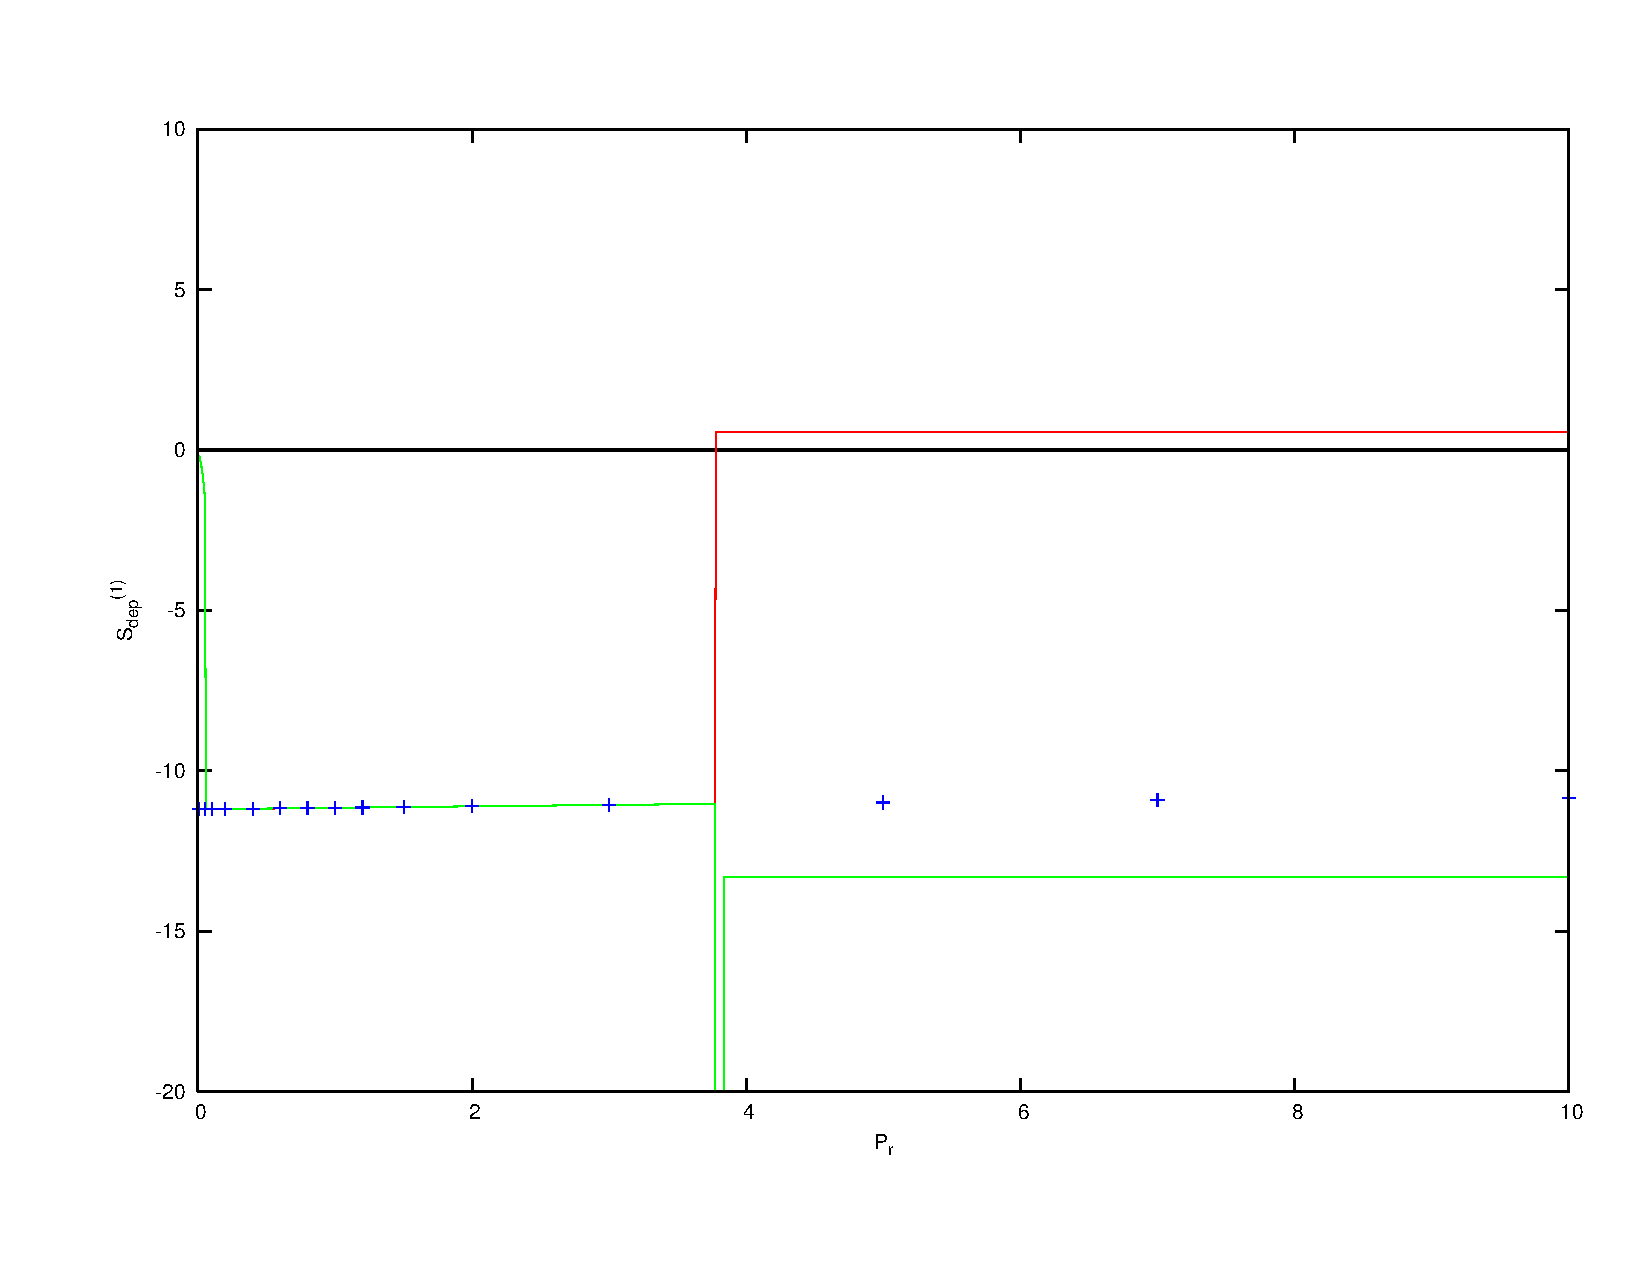
\includegraphics[trim = 1.5cm 2cm 0 1cm, clip = true, width=14cm]{Sdep1Tc050}
	\caption{$S_{dep}^{(1)}$ as a function of reduced pressure, for $T_r = 0.500$. Line plots show computational results with phase set to liquid (red) and gas (green), respectively. Data points show the negatives of tabulated values from Table 10 in \cite{LK}}
	\label{fig:Sdep1Tc050}
\end{figure}

The departure entropy for simple fluid calculations are given in Figure \ref{fig:Sdep0Tc050}, for reduced temperature $T_r = 0.500$. The results are in agreement with the tabulated values, for the pressure interval that give the correct reduced specific volume. However, since the reduced temperature is lower, than that in Figures \ref{fig:z0Tc090} and \ref{fig:z1Tc090}, the reduced specific volume calculations are constrained to a more narrow interval ($P_r < 3.8$). The results for $S_{dep} ^{(1)}$, given in Figure \ref{fig:Sdep1Tc050} share these characteristics.

\subsubsection*{Departure enthalpy}
The departure enthalpy $H_{dep}^{(0)}$ and  $H_{dep}^{(1)}$, for reduced temperature $T_r = 1.300$ is plotted in Figures \ref{fig:Hdep0Tc130} and \ref{fig:Hdep1Tc130}, respectively. The computational results are in exact agreement with the tabulated values, for the entire pressure interval in the figures. Again, this is due to the choice of reduced temperature. A high reduced temperature allows for accurate calculations of the reduced specific volume, even for high pressures. The reduced pressure $P_r = 10.000$ equals an actual pressure of 579 bar, for this specific fluid mixture.

\begin{figure}[h]
	\centering
	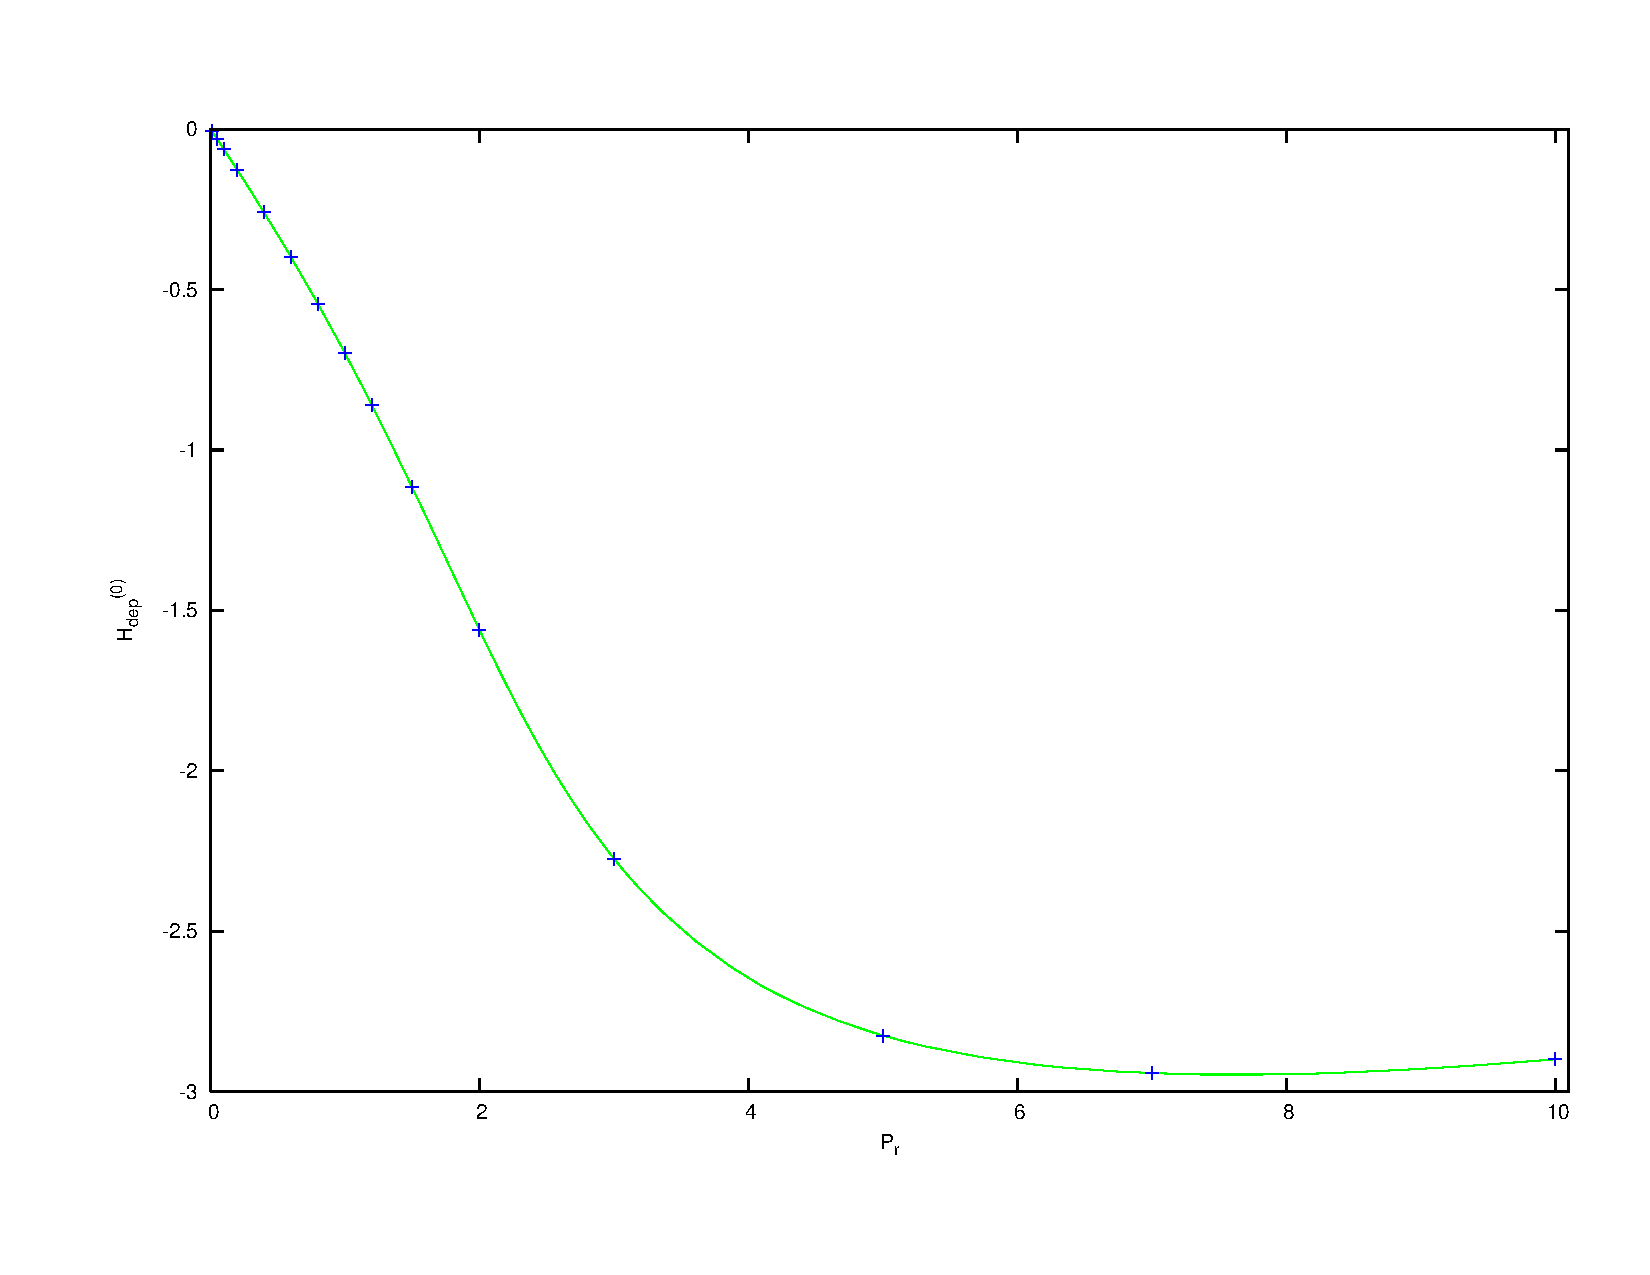
\includegraphics[trim = 1.5cm 2cm 0 1cm, clip = true, width=14cm]{Hdep0Tc130}
	\caption{$H_{dep}^{(0)}$ as a function of reduced pressure, for $T_r = 1.300$. Line plots show computational results with phase set to liquid (red) and gas (green), respectively. Curves overlap in the entire pressure interval. Data points show the negatives of tabulated values from Table 7 in \cite{LK}}
	\label{fig:Hdep0Tc130}
\end{figure}


\begin{figure}
	\centering
	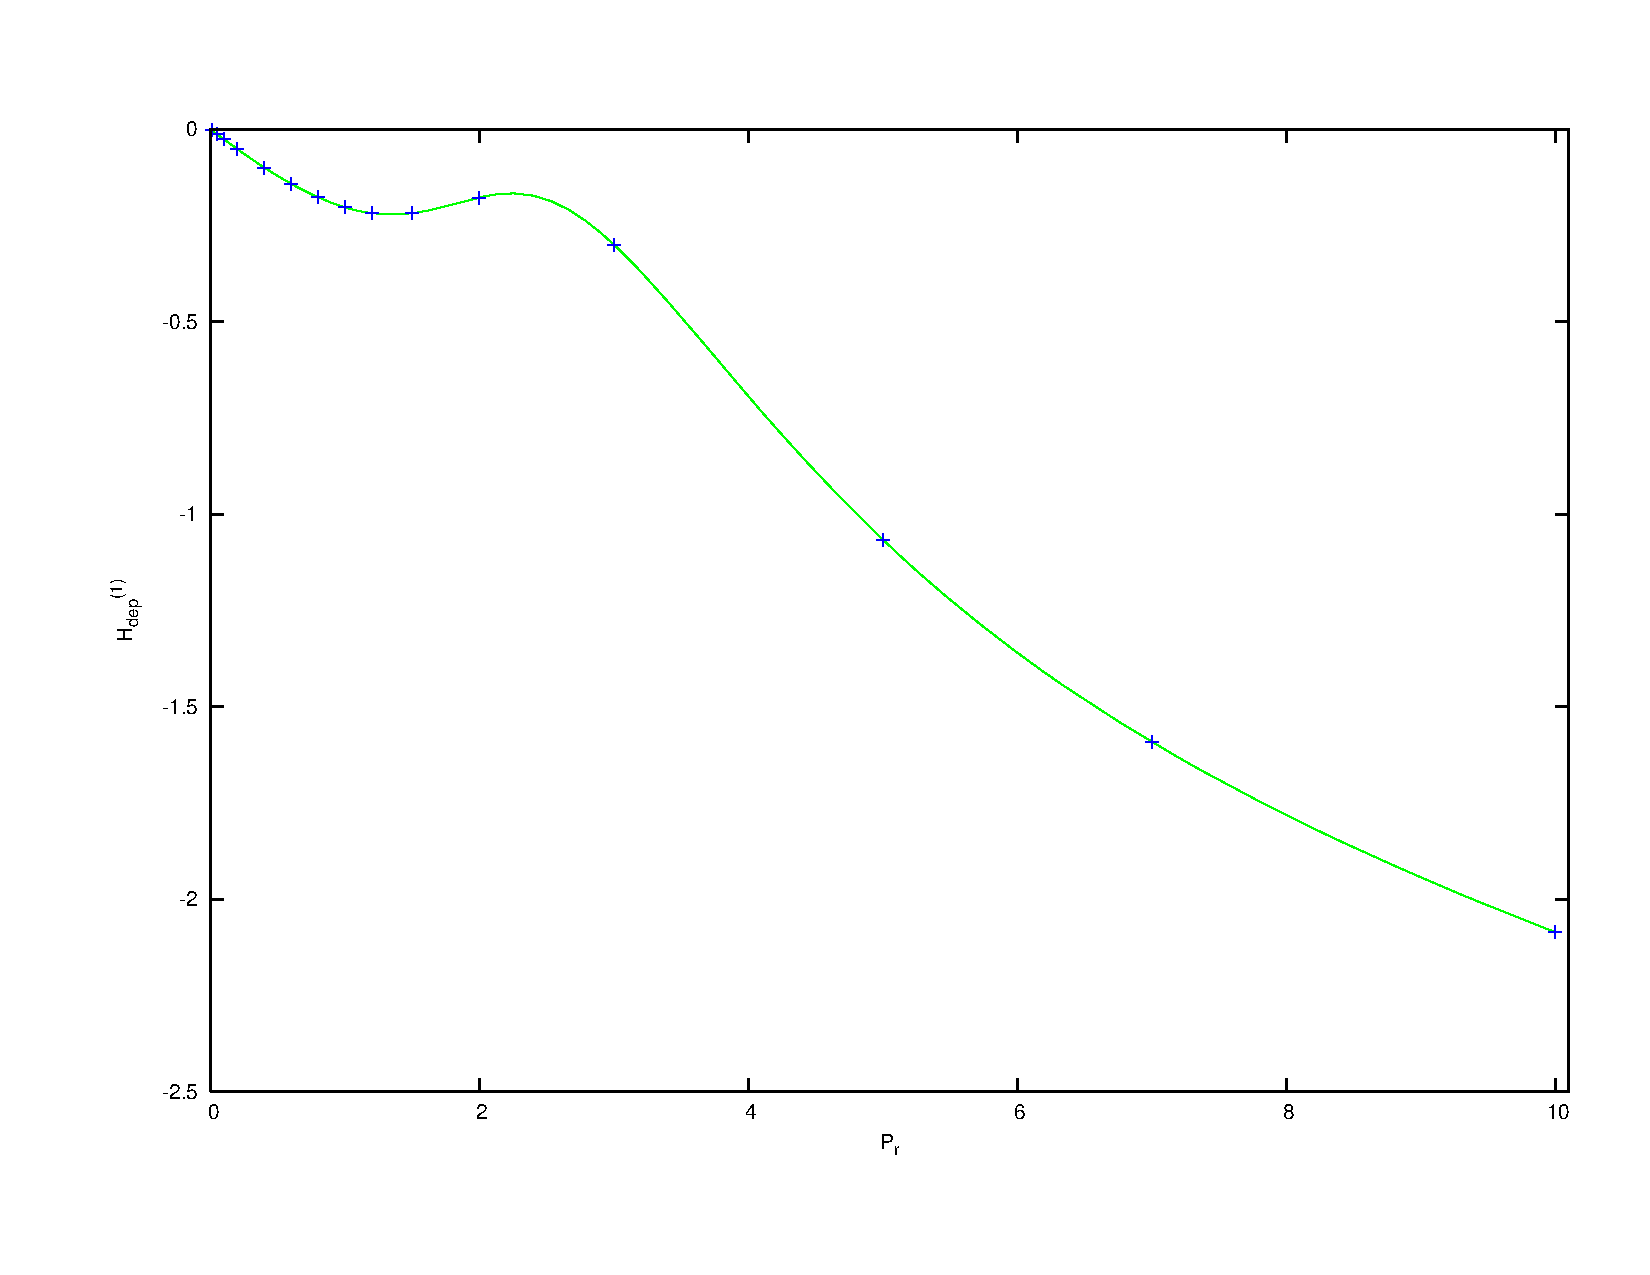
\includegraphics[trim = 1.5cm 2cm 0 1cm, clip = true, width=13cm]{Hdep1Tc130}
	\caption{$H_{dep}^{(1)}$ as a function of reduced pressure, for $T_r = 1.300$. Line plots show computational results with phase set to liquid (red) and gas (green), respectively. Curves overlap in the entire pressure interval. Data points show the negatives of tabulated values from Table 8 in \cite{LK}}
	\label{fig:Hdep1Tc130}
\end{figure}

\subsection{Computational comparison of fugacity coefficients}
To have some reasonable values to compare the component fugacity coefficients to, an implementation of the Soave-Redlich-Kwong (SRK) equation of state, is used. Component fugacity coefficients are computed for the same mixture, and the same reduced temperatures, as used in the Subsection \ref{subsec:dircomp}. Pressures range from $P_r = 0.010$ to $P_r = 5.000$. The results calculated with the Lee-Kesler implementation, and the results calculated by use of the SRK equation of state are plotted together in Figures \ref{fig:fug05Tc}, \ref{fig:fug09Tc} and \ref{fig:fug13Tc}, for $T_r = 0.500$, $T_r = 0.900$ and $T_r = 1.300$, respectively.

\begin{figure}
	\centering
	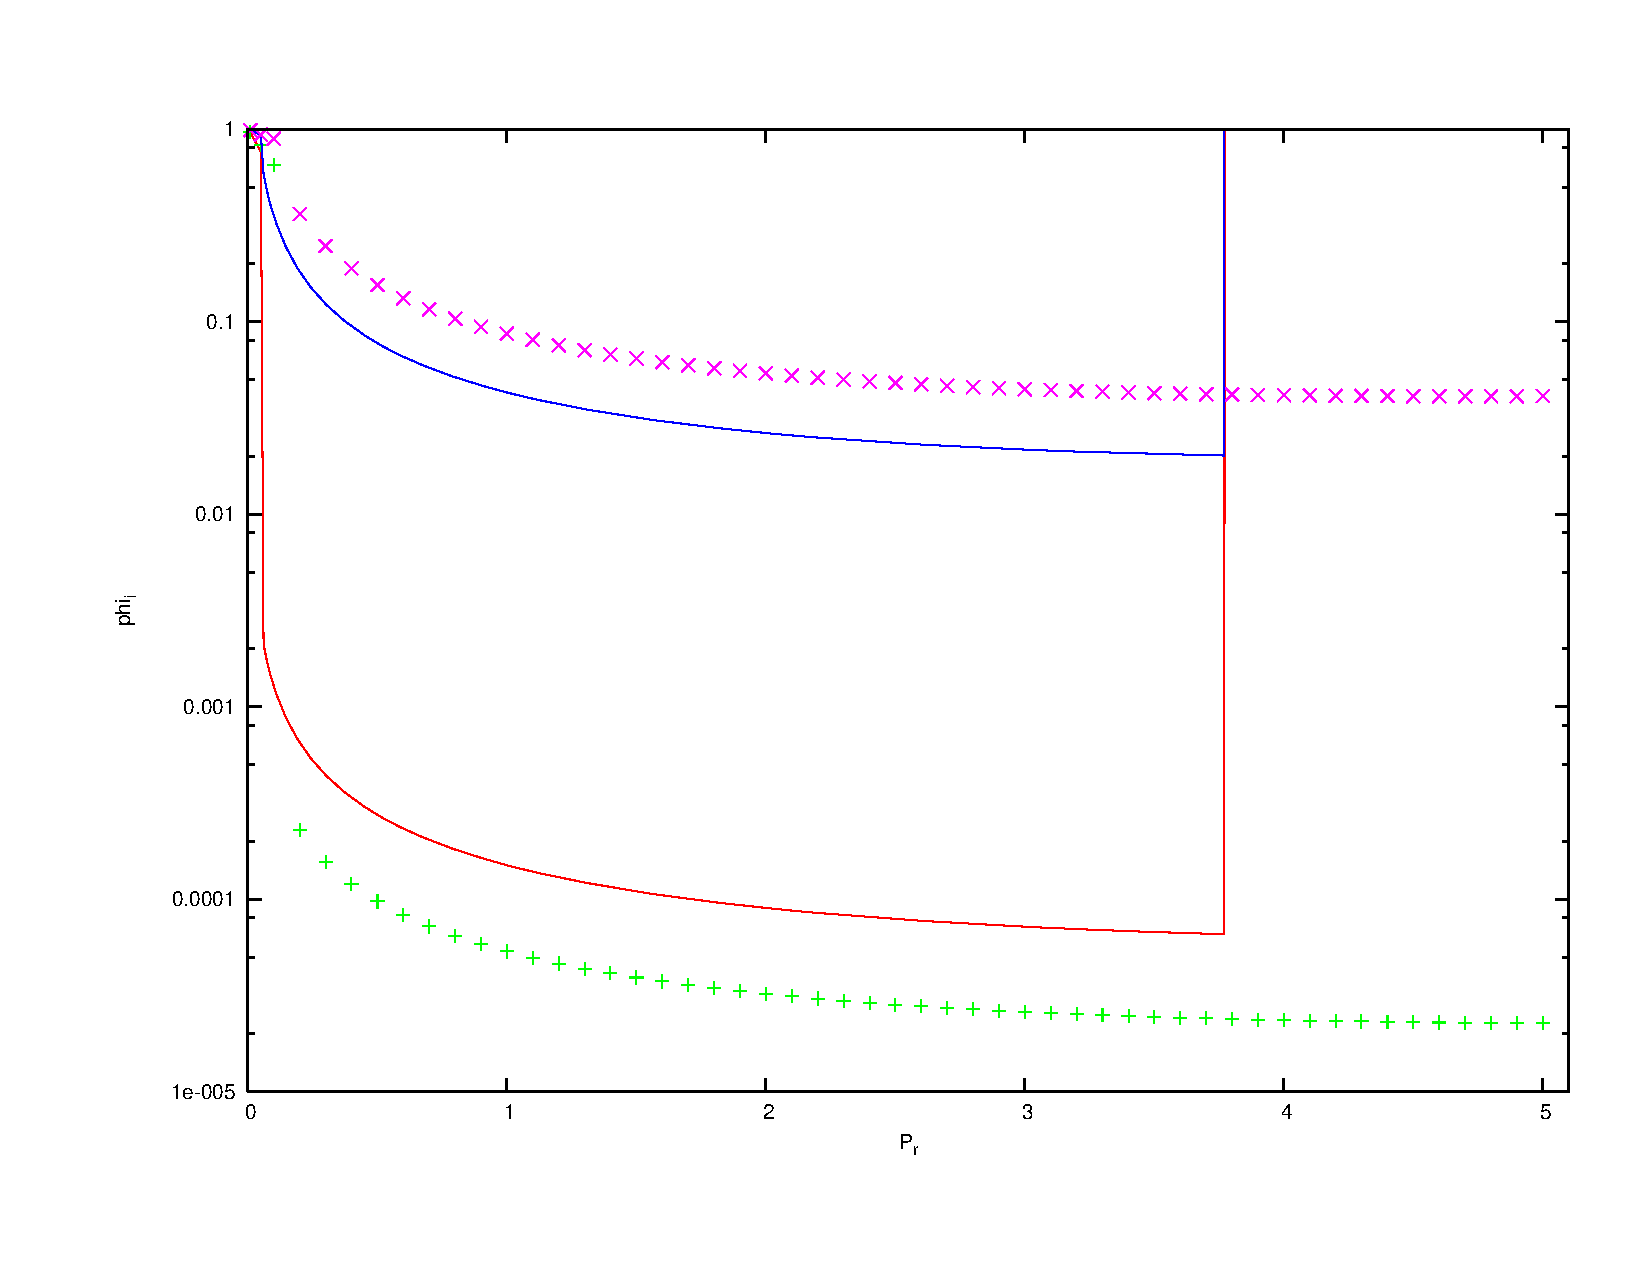
\includegraphics[trim = 1.5cm 2cm 0 1cm, clip = true, width=13cm]{fug05Tc}
	\caption{Fugacity coefficients $\phi_i$ as a function of reduced pressure $P_r$, for $T_r = 0.500$. Line plots show computational results done by the Lee-Kesler method, and data point represent computational results done by calculations with the SRK equation of state. Red curve/green data points represent CO$_2$ component, blue curve/pink data points represent methane component.}
	\label{fig:fug05Tc}
\end{figure}

\begin{figure}
	\centering
	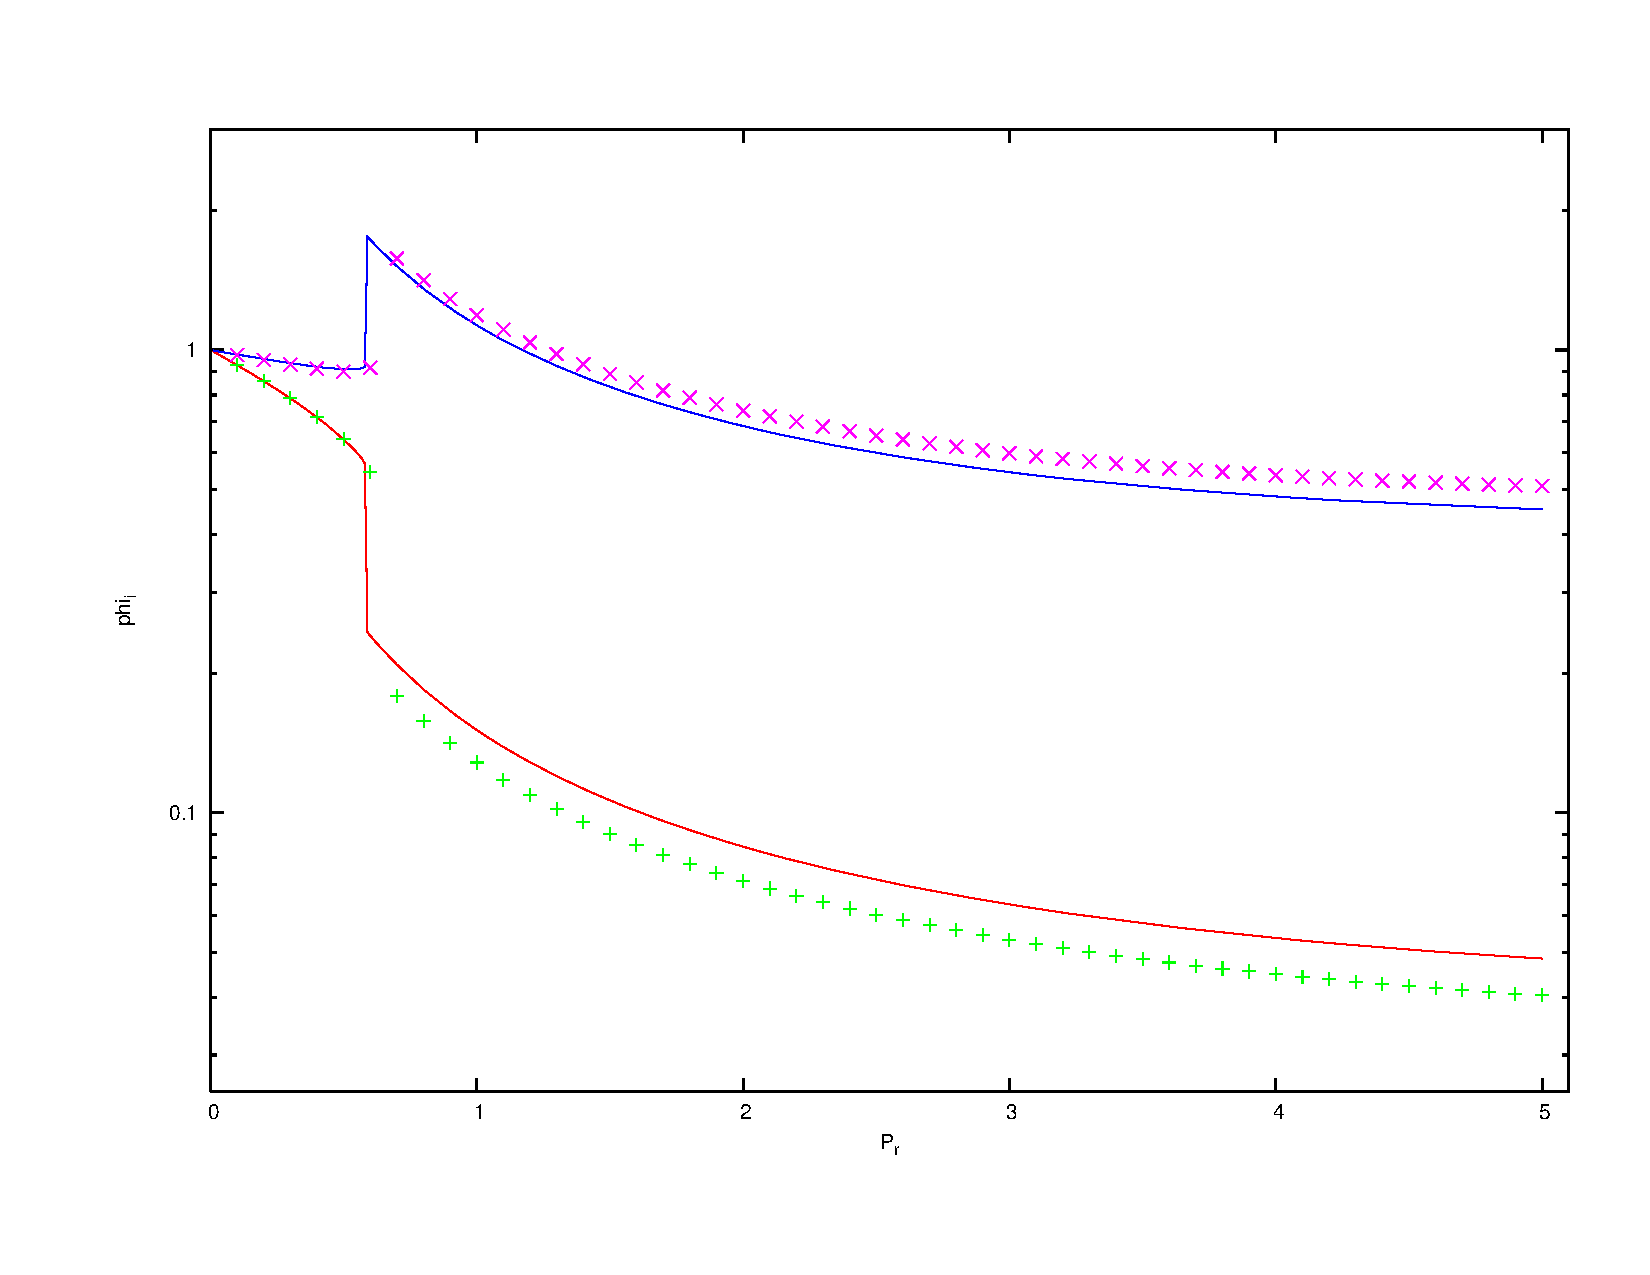
\includegraphics[trim = 1.5cm 2cm 0 1cm, clip = true, width=12.5cm]{fug09Tc}
	\caption{Fugacity coefficients $\phi_i$ as a function of reduced pressure $P_r$, for $T_r = 0.500$. Line plots show computational results done by the Lee-Kesler method, and data point represent computational results done by calculations with the SRK equation of state. Red curve/green data points represent CO$_2$ component, blue curve/pink data points represent methane component.}
		\label{fig:fug09Tc}
\end{figure}

\begin{figure}
	\centering
	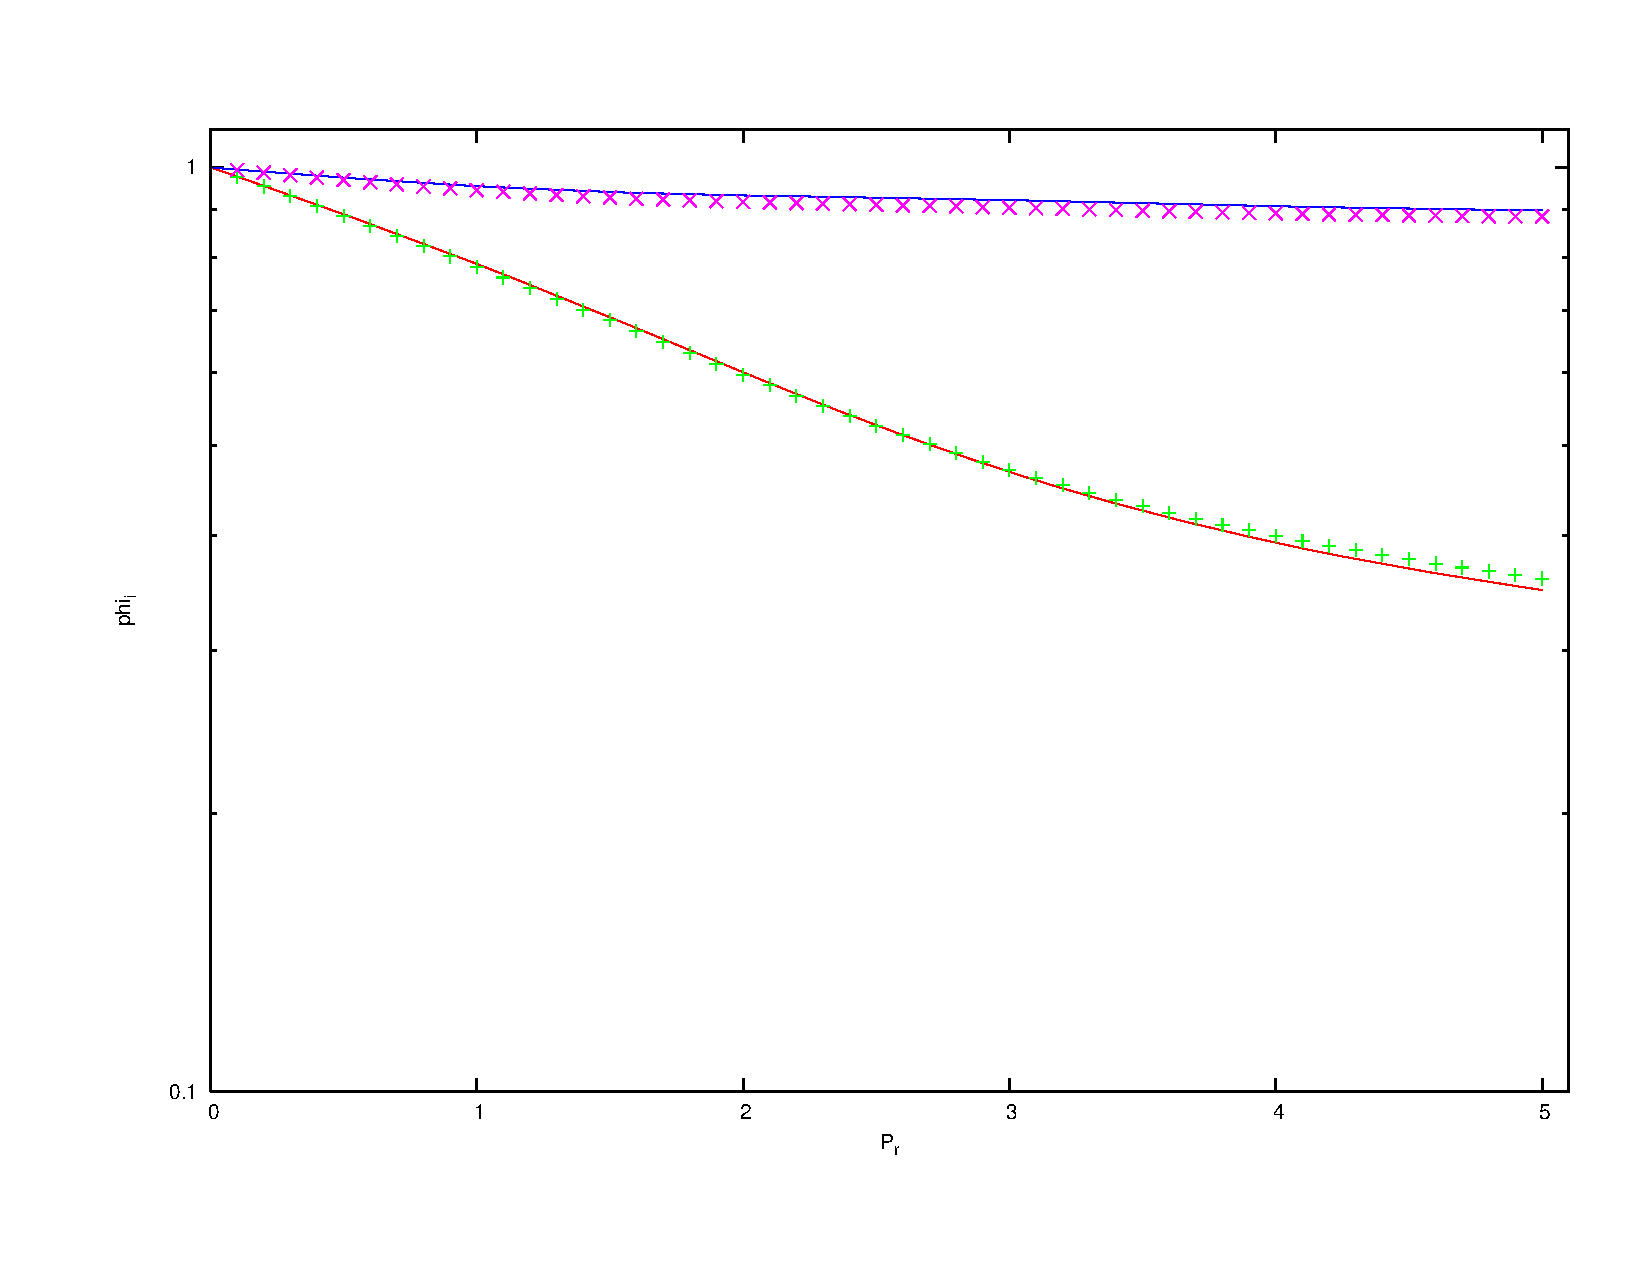
\includegraphics[trim = 1.5cm 2cm 0 1cm, clip = true, width=12.5cm]{fug13Tc}
	\caption{Fugacity coefficients $\phi_i$ as a function of reduced pressure $P_r$, for $T_r = 0.500$. Line plots show computational results done by the Lee-Kesler method, and data point represent computational results done by calculations with the SRK equation of state. Red curve/green data points represent CO$_2$ component, blue curve/pink data points represent methane component.}
	\label{fig:fug13Tc}
\end{figure}

The plots show that the fugacity coefficients for the two different thermodynamic models behave similarly, even though there is some deviation in the numerical values. The largest relative deviation is the temperature, $T_r = 0.500$ ($T = 118$ K). But, if only pressures below the threshold that yields inaccurate reduced specific volume vales, these results look quite good. To get a better understanding of the actual precision of the numerical calculations done with this implementation, accurate experimental results should be used for comparison.

\section{Conclusion and further work}
The main challenge in the implementation of the Lee-Kesler model is solving the Lee-Kesler equation of state, with respect to the reduced specific volume. The equation to be solved is a high order non-linear equation, with exponential damping, with particular roots that corresponds to particular physical phases of the fluid studied. In solving this equation, a routine written by Anders Austegard has been used, with some modifications to be more robust in choosing correct phase. The results are satisfactory in certain temperature and pressure ranges, but not good enough to be trusted in general. Problems arise for states where the reduced pressure is much larger than the reduced temperature. A discontinuity in the computed thermodynamic properties results can clearly be seen in Figures \ref{fig:z0Tc090}, \ref{fig:z1Tc090}, \ref{fig:Sdep0Tc050}, \ref{fig:Sdep1Tc050} and \ref{fig:fug05Tc}. This is discontinuity is a direct consequence of the reduced volume solver not finding an accurate result. It is recommended to take a closer look at the behaviour of $f$ given by Equation \ref{eq:fv}, for high reduced pressure to reduced temperature ratios, to get a better understanding of the reduced specific volume for these states. This will hopefully help constructing a more general solver for the equation.

Despite the challenges posed by the reduced volume, the implementation of the Lee-Kesler model, with the modern Helmholtz function approach has been successful. The thermodynamic properties compressibility factor, entropy departure and enthalpy departure, yield identical results by this method, as by the original implementation, in the region where the volume is accurate. 

Take note of the following: Even if the modern method was not used to find these values, but instead the Equations in \cite{LK}, inaccurate reduced specific volume values would result in deviations just the same. The modern approach does not introduce any new errors in the implementation, but gives a large range of consistency test, to check derivatives used in the implementation. In addition, with small additions in the program, other thermodynamic properties can easily be calculated. This includes Gibbs free energy and heat capacities, which can be found expressed by the Helmholtz function $F$, and its partial derivatives in \cite{MM}. Since these are already implemented in the module, the modification is straightforward, and does not require more than a few lines of code.

The component fugacity coefficients have been calculated and compared to similar calculations done with the Soave-Redlich-Kwong equation of state. The behaviour of these coefficients are similar in the two models, but the relative deviation increases as the reduced temperature is lowered. 
None of the thermodynamic properties have been compared to experimental results. This is highly recommended, before taking the module into use.

\clearpage
\begin{thebibliography}{9}
  
\bibitem{LK}
	Lee, B.I., Kesler, M.G., \textit{A Generalized thermodynamic correlation based on a three-parameter corresponding states}, AlChE Journal, 21 (3), 510 (1975)

\bibitem{PKP}
	Plocker, U., Knapp, H., Prausnitz, J., \textit{Calculations of High-Pressure Vapor-Liquid Equilibria from a Corresponding-States Correlation with Emphasis on Asymmetric Mixtures}, Ind. Eng. Chem. Process Des. Dev, 17 (3) 324 (1978)
	
\bibitem{MM}
	Michelsen, M. L., Mollerup, J. M., \textit{Thermodynamic Models: Fundamentals \& computational aspects}, second edition, Tie-Line Publications (2007)

%\bibitem{HSA}
%	Hammer, M., Skaugen, G., Aursand, E., \textit{Memo: Introduction to thermodynamics}, SINTEF Energi A%S, 2013

\end{thebibliography}

\clearpage
\appendix

\section{The triple product rule}
\label{app:tripProdRule}
The triple product rule, is a formula which relates partial derivatives of three interdependent variables. That is, partial derivatives of functions of three variables, where each variable is given as an implicit function of the two other variables. For a function $f = f(x,y,z)$ with interdependent variables, the partial derivatives of the variables are related by:
\begin{equation}
\label{def:tripProdRule}
\pder{x}{y}_z \pder{y}{z}_x \pder{z}{x}_y = -1
\end{equation}
The subscripts indicate which of the variables are held constant when the partial derivative is taken.

\subsubsection*{Partial volume derivatives}
In thermodynamics, pressure, temperature, volume and composition may be expressed as dependent on each other. Therefore, three of these variables is enough to decide the last one (for a given phase). Hence, if we let $f = T$ and $x,y,z = V,P,\textbf{n}$, and insert into Equation \reff{def:tripProdRule} we get:
\begin{equation}
\pder{V}{P}_{n_i} \pder{P}{n_i}_V \pder{n_i}{V}_P = -1
\end{equation}

By rewriting this, we find the partial derivative of the volume, with respect to composition, for fixed pressure, expressed in terms of the pressure derivatives:
\begin{equation}
\pder{V}{n_i}_P = - \frac{\pder{P}{n_i}_V}{\pder{P}{V}_{n_i}}
\end{equation}

Similarly, if we insert $f = n_i$ and $x,y,z = V,P,T$ into Equation \reff{def:tripProdRule} we get:
\begin{equation}
\pder{V}{P}_{T} \pder{P}{T}_V \pder{T}{V}_P = -1
\end{equation}

By rewriting this, we find the partial derivative of the volume, with respect to temperature, for fixed pressure, expressed in terms of the pressure derivatives:
\begin{equation}
\pder{V}{T}_P = - \frac{\pder{P}{T}_V}{\pder{P}{V}_{T}}
\end{equation}

\section{Partial derivatives of thermodynamic properties}
\label{app:partDerivatives}
In this appendix section, thorough derivations for the partial derivatives of the thermodynamic properties of interest are presented. In these derivations, Equations \reff{def:P} - \reff{def:V_T} are used to simplify notation.
\subsection{Compressibility}
Partial derivative of the compressibility with respect to temperature:
\begin{equation}
\begin{split}
\left( \frac{\partial z}{\partial T} \right)_{P, \textbf{n}}
& = \left( \frac{\partial }{\partial T} \frac{PV}{nRT}\right)_{P, \textbf{n}} \\
& = - \frac{PV}{nRT^2} + \frac{P}{nRT} \left( \frac{\partial V}{\partial T} \right)_{P, \textbf{n}} \\
& = - \frac{z}{T} + \frac{z}{V} \left( \frac{\partial V}{\partial T} \right)_{P, \textbf{n}} \\
& = -z\left[\frac{1}{T} - \frac{\bar{V}_T}{V}\right]
\end{split}
\end{equation}

Partial derivative of the compressibility with respect to pressure:
\begin{equation}
\begin{split}
\left( \frac{\partial z}{\partial P} \right)_{T, \textbf{n}}
& = \left( \frac{\partial }{\partial P} \frac{PV}{nRT} \right)_{T, \textbf{n}} \\
& = \frac{V}{nRT} + \frac{P}{nRT} \left( \frac{\partial V}{\partial P} \right)_{T, \textbf{n}} \\
& = \frac{z}{P} + \frac{z}{V} \left( \frac{\partial V}{\partial P} \right)_{T, \textbf{n}} \\
& = z \left[ \frac{1}{P} + \frac{1}{V \pder{P}{V}_{T,\textbf{n}}} \right]
\end{split}
\end{equation}

Partial derivative of the compressibility with respect to composition:
\begin{equation}
\begin{split}
\left( \frac{\partial z}{\partial n_i} \right)_{T,P}
& = \left( \frac{\partial }{\partial n_i} \frac{PV}{nRT} \right)_{T,P} \\
& = - \frac{PV}{n^2RT} + \frac{P}{nRT} \left( \frac{\partial V}{\partial n_i} \right)_{T,P} \\
& = - z \left[ \frac{1}{n} - \frac{\bar{V}_i}{V}  \right]
\end{split}
\end{equation}

\subsection{Entropy}

Partial derivative of entropy with respect to temperature:
\begin{equation}
\begin{split}
\left( \frac{\partial S^R(T,P,\textbf{n})}{\partial T} \right)_{P,\textbf{n}}
& = \left( \frac{\partial S^R(T,V, \textbf{n})}{\partial T} \right)_{P,\textbf{n}} + \left( \frac{\partial nR \ln z}{\partial T} \right)_{P,\textbf{n}} \\
& = \pder{S^R(T,V,\textbf{n})}{T}_{V,\textbf{n}} \pder{T}{T}_{P,\textbf{n}} + \pder{S^R(T,V,\textbf{n})}{V}_{T,\textbf{n}} \\
& \qquad \qquad \cdot \pder{V}{T}_{P,\textbf{n}} + \frac{nR}{z} \pder{z}{T}_{P,\textbf{n}} \\
& = \pder{S^R(T,V,\textbf{n})}{T}_{V,\textbf{n}} - \pder{S^R(T,V,\textbf{n})}{V}_{T,\textbf{n}} \frac{\pder{P}{T}_{V,\textbf{n}}}{\pder{P}{V}_{T,\textbf{n}}} \\
& \qquad \qquad + \frac{nR}{z} \pder{z}{T}_{P,\textbf{n}} 
\end{split}
\end{equation}

Partial derivative of entropy with respect to pressure:
\begin{equation}
\begin{split}
\left( \frac{\partial S^R(T,P,\textbf{n})}{\partial P} \right)_{T,\textbf{n}}
& = \left( \frac{\partial S^R(T,V, \textbf{n})}{\partial P} \right)_{T,\textbf{n}} + \left( \frac{\partial nR \ln z}{\partial P} \right)_{T,\textbf{n}} \\
& = \pder{S^R(T,V,\textbf{n})}{V}_{T,\textbf{n}} \frac{1}{\pder{P}{V}_{T,\textbf{n}}} + \frac{nR}{z} \pder{z}{P}_{T,\textbf{n}}
\end{split}
\end{equation}

Partial derivative of entropy with respect to composition:
\begin{equation}
\begin{split}
\left( \frac{\partial S^R(T,P,\textbf{n})}{\partial n_i} \right)_{T,P}
& = \left( \frac{\partial S^R(T,V, \textbf{n})}{\partial n_i} \right)_{T,P} + \left( \frac{\partial nR \ln z}{\partial n_i} \right)_{T,P} \\
& = \pder{S^R(T,V,\textbf{n})}{V}_{T,\textbf{n}} \pder{V}{n_i}_{T,P} + \pder{S^R(T,V,\textbf{n})}{n_i}_{V,T} \\
& \qquad \qquad \cdot \pder{n_i}{n_i}_{T,P} + \frac{nR}{z} \pder{z}{n_i}_{T,P} + R \ln z\\
& = \pder{S^R(T,V,\textbf{n})}{V}_{T,\textbf{n}} \bar{V}_i + \pder{S^R(T,V,\textbf{n})}{n_i}_{V,T} \\
& \qquad \qquad  + \frac{nR}{z} \pder{z}{n_i}_{T,P} + R \ln z
\end{split}
\end{equation}

The derivatives of $S^R(T,V,\textbf{n})$ in these equations can be found by differentiating Equation \reff{def:S^R(T,V,n)}:
\begin{align}
\label{eq:S^R_T_TVn}
& \pder{S^R(T,V,\textbf{n})}{T}_{V,\textbf{n}} = -R \left[2 \pder{F}{T}_{V,\textbf{n}} + T\pdder{F}{T}_{V,\textbf{n}} \right] \\
& \pder{S^R(T,V,\textbf{n})}{V}_{T,\textbf{n}} = -R \left[\pder{F}{V}_{T,\textbf{n}} + T \pdcross{F}{T}{V}_\textbf{n} \right] \\ 
\label{eq:S^R_ni_TVn}
& \pder{S^R(T,V,\textbf{n})}{n_i}_{V,T} = -R \left[\pder{F}{n_i}_{V,T} + T \pdcross{F}{T}{n_i}_V \right]
\end{align}
 
By use of Equations \ref{eq:S^R_T_TVn} - \ref{eq:S^R_ni_TVn}, together with Equations Equations \reff{def:P} - \reff{eq:z_i}, the expressions for the derivatives of the reduced entropy can be simplified to:
\begin{align}
& \pder{S^R(T,P,\textbf{n})}{T}_{P,\textbf{n}} = \bar{V}_T \pder{P}{T}_{V,\textbf{n}} - R \left[2\pder{F}{T}_{V,\textbf{n}} + T \pdder{F}{T}_{V,\textbf{n}} + \frac{n}{T} \right] \\
& \pder{S^R(T,P,\textbf{n})}{P}_{T,\textbf{n}} = \frac{nR}{P} - \bar{V}_T \\
& \pder{S^R(T,P,\textbf{n})}{n_i}_{T,P} = \bar{V}_i \pder{P}{T}_{V,\textbf{n}} - R\left[ \pder{F}{n_i}_{T,V} + T\pdcross{F}{T}{n_i}_V + 1 - \ln z \right] 
\end{align}
\subsection{Enthalpy}
Partial derivative of enthalpy with respect to temperature:
\begin{equation}
\begin{split}
\pder{H^R}{T}_{P, \textbf{n}} & = \pder{A^R(T,V,\textbf{n})}{T}_{P, \textbf{n}} + S^R(T,V,\textbf{n}) + T \pder{S^R(T,V,\textbf{n})}{T}_{P, \textbf{n}} \\
& \qquad \qquad + P \pder{V}{T}_{P,\textbf{n}} - nR \\
& = \pder{A^R}{T}_{V,\textbf{n}} +\pder{V}{T}_{P,\textbf{n}} \left[ \pder{A^R}{V}_{T,\textbf{n}} + T \pder{S^R(T,V,\textbf{n})}{V}_{T,\textbf{n}} + p \right] \\
& \qquad \qquad - \pder{A^R}{T}_{P,\textbf{n}} + T\pder{S^R(T,V,\textbf{n})}{T}_{V,\textbf{n}} - nR \\
& = \bar{V}_T T \pder{P}{T}_{V,\textbf{n}} - RT \left[ 2\pder{F}{T}_{V,\textbf{n}} + T \pdder{F}{T} + \frac{n}{T} \right]
\end{split}
\end{equation}

Partial derivative of enthalpy with respect to pressure:
\begin{equation}
\begin{split}
\pder{H^R}{P}_{T, \textbf{n}} & =  \pder{A^R(T,V,\textbf{n})}{P}_{T, \textbf{n}} + T \pder{S^R(T,V,\textbf{n})}{P}_{T, \textbf{n}} + V + P \pder{V}{P}_{T,\textbf{n}} \\
& = \left[ RT \pder{F}{V}_{T,\textbf{n}} + T \pder{S^R(T,V,\textbf{n})}{V}_{T,\textbf{n}} + P \right] \pder{V}{P}_{T,\textbf{n}} + V \\
& = \left[- RT^2 \pdcross{F}{T}{V}_{\textbf{n}}  + P \right] \pder{V}{P}_{T,\textbf{n}} + V \\
& = V - T \bar{V}_T
\end{split}
\end{equation}

Partial derivative of enthalpy with respect to composition:
\begin{equation}
\begin{split}
\pder{H^R}{n_i}_{T,P} & = \pder{A^R(T,V,\textbf{n})}{n_i}_{T,P} + T \pder{S^R(T,V,\textbf{n})}{n_i}_{T,P} + P \pder{V}{n_i}_{T,P} - RT \\
& = \bar{V}_i \left[ RT \pder{F}{V}_{T,n_i} + T \pder{S^R(T,V,\textbf{n})}{V}_{T,\textbf{n}} + P \right] + RT\pder{F}{n_i}_{T,V}  \\
& \qquad \qquad  + T\pder{S^R(T,V,\textbf{n})}{n_i}_{T,V}  - RT \\
& = \bar{V}_i T \pder{P}{T}_{V,\textbf{n}} -RT^2 \pdcross{F}{T}{n_i}_V - RT
\end{split} 
\end{equation}

\subsection{Fugacity coefficients}
Partial derivative of fugacity coefficients with respect to temperature:
\begin{equation}
\begin{split}
\pder{\ln \phi_i}{T}_{P, \textbf{n}} 
& = \left(\pd{}{T} \pder{F}{n_i}_{T,V} \right)_{P, \textbf{n}} - \pder{\ln z}{T}_{P,\textbf{n}} \\
& = \pdcross{F}{T}{n_i}_V + \pdcross{F}{V}{n_i}_{T} \pder{V}{T}_{\textbf{n}}- \frac{1}{z}\pder{z}{T}_{P, \textbf{n}} \\
& = \pdcross{F}{T}{n_i}_V - \pdcross{F}{V}{n_i}_{T} \frac{\pder{P}{T}_{V,\textbf{n}}}{\pder{P}{V}_{T,\textbf{n}}} + \frac{1}{T} + \frac{1}{V} \frac{\pder{P}{T}_{V,\textbf{n}}}{\pder{P}{V}_{T,\textbf{n}}} \\
& = \pdcross{F}{T}{n_i}_V + \frac{1}{T} + \frac{\pder{P}{T}_{V,\textbf{n}}}{\pder{P}{V}_{T,\textbf{n}}} \left[\frac{1}{V} - \pdcross{F}{V}{n_i}_{T} \right] \\
& = \pdcross{F}{T}{n_i}_V + \frac{1}{T} + \frac{\pder{P}{T}_{V,\textbf{n}}}{\pder{P}{V}_{T,\textbf{n}}} \frac{1}{RT} \pder{P}{n_i}_{T,V} \\
& = \pdcross{F}{T}{n_i}_V + \frac{1}{T} - \frac{\bar{V}_i}{RT}  \pder{P}{T}_{V,\textbf{n}} 
\end{split}
\end{equation}

Partial derivative of fugacity coefficients with respect to pressure:
\begin{equation}
\begin{split}
\pder{\ln \phi_i}{P}_{T, \textbf{n}} 
& = \left(\pd{}{P} \pder{F}{n_i}_{T,V} \right)_{T, \textbf{n}} - \pder{\ln z}{P}_{T,\textbf{n}} \\
& = \pdcross{F}{V}{n_i}_{T} \pder{V}{P}_{T, \textbf{n}} - \frac{1}{z} \pder{z}{P}_{T,\textbf{n}} \\
& = \frac{1}{\pder{P}{V}_{T,\textbf{n}}} \left[ \pdcross{F}{V}{n_i}_{T} - \frac{1}{V} \right] - \frac{1}{P} \\
& = \frac{\bar{V}_i}{RT} - \frac{1}{P} 
\end{split}
\end{equation}

Partial derivative of fugacity coefficients with respect to composition:
\begin{equation}
\begin{split}
\pder{\ln \phi_i}{n_j}_{T, P} 
& = \left(\pd{}{n_j} \pder{F}{n_i}_{T,V} \right)_{T, P} - \pder{\ln z}{n_j}_{T,P} \\
& = \pdcross{F}{V}{n_i}_{T,\textbf{n}} \pder{V}{n_j}_{T,P} + \pdcross{F}{n_j}{n_i}_{T,P} - \frac{1}{z} \pder{z}{n_j}_{T,P} \\
& = \pdcross{F}{V}{n_i}_{T,\textbf{n}} \pder{V}{n_j}_{T,P} + \pdcross{F}{n_j}{n_i}_{T,P} + \frac{1}{n} - \frac{\bar{V}_j}{V} \\
& = \pdcross{F}{n_j}{n_i}_{T,P} + \frac{1}{n} + \bar{V}_j \left[\pdcross{F}{V}{n_i}_{T,\textbf{n}} - \frac{1}{V} \right] \\
& = \pdcross{F}{n_j}{n_i}_{T,P} + \frac{1}{n} + \frac{\pder{P}{V}_{T,\textbf{n}}}{RT} \bar{V}_j \bar{V}_i \\
\end{split}
\end{equation}

\section{Constants for simple fluid and reference fluid}
\label{app:constants}
\begin{table}[h!]
\begin{center}
\caption{Constants that separate calculations for simple and reference fluid}
\label{tab:constants}
\begin{tabular}{c c c}
\hline
Constant & Simple fluid & Reference fluid \\
\hline
$b_1$	& 0.1181193	& 0.2026579 \\
$b_2$ 	& 0.265728	& 0.331511	\\
$b_3$	& 0.154790 	& 0.203488	\\
$b_4$	& 0.030323 	& 0.203488 	\\
$c_1$	& 0.0236744	& 0.0313385	\\
$c_2$	& 0.0186984 & 0.0503618	\\
$c_3$	& 0.0		& 0.016901	\\
$c_4$	& 0.042724	& 0.041577	\\
$d_1 \cdot 10^4$	& 0.155488  & 0.48736 	\\
$d_2 \cdot 10^4$	& 0.623689 	& 0.0740336\\
$\beta$	& 0.65392	& 1.226		\\
$\gamma$& 0.060167	& 0.03754	\\
\hline
\end{tabular}
\end{center}
\end{table}

\section{Solving the Helmholtz function integral for the Lee-Kesler model}
\label{app:integral}
The integral at hand is:

\begin{equation}
F(T,V,\textbf{n}) = - n \int_\infty ^V \frac{1}{V'} \left[\frac{B}{v_r '} + \frac{C}{(v_r ') ^2 } + \frac{D}{(v_r ')^5} + \frac{E}{(v_r ')^2} \left( \beta + \frac{\gamma}{(v_r ')^2} \right) \exp{\left(-\frac{\gamma}{(v_r ')^2}\right)} \right] \mathrm{d}V'
\end{equation}

By changing integration variable from $V'$ to $u = v_r ' = \dfrac{P_{cM} V'}{n R T_{cM}}$ this can be written in a more convenient form:

\begin{equation}
F(T,V,\textbf{n}) = - n \int_\infty ^{v_r} \left[\frac{B}{u^2} + \frac{C}{u^3} + \frac{D}{u^6} + \frac{E}{u^3} \left( \beta + \frac{\gamma}{u^2} \right) \exp{\left(-\frac{\gamma}{u^2}\right)} \right] \mathrm{d}u
\end{equation}

The tricky part of this integral is the exponential term. For convenience we separate the integral into three parts:
\begin{equation}
F(T,V,\textbf{n}) = I_1 + I_2
\end{equation}

where

\begin{align}
& I_1 = - n \int_\infty ^{v_r} \left(\frac{B}{u^2} + \frac{C}{u^3} + \frac{D}{u^6} \right) \mathrm{d}u \\
& I_2 = - n \int_\infty ^{v_r} \frac{E}{u^3} \left(\beta + \frac{\gamma}{u^2} \right) \exp{\left(-\frac{\gamma}{u^2}\right)}  \mathrm{d}u
\end{align}

The first of these can be solved straightforward:
\begin{equation}
I_1 = n \left(\frac{B}{v_r} + \frac{C}{2 v_r^2} + \frac{D}{5 v_r^5} \right)
\end{equation}

When solving the second integral, consider the exponential factor:
\begin{align}
& \left( \pd{}{u} \exp{\left(-\frac{\gamma}{u^2} \right) } \right)= \frac{2 \gamma}{u^3} \exp{\left(-\frac{\gamma}{u^2} \right) }\\
& \left( \pd{}{\gamma} \exp{\left(-\frac{\gamma}{u^2} \right) } \right) = - \frac{1}{u^2}\exp{\left(-\frac{\gamma}{u^2} \right) } \\
& \left(\frac{\partial^2}{\partial u \partial \gamma} \exp{\left(-\frac{\gamma}{u^2}\right)} \right) = \left(\frac{2}{u^3} - \frac{2\gamma}{u^5}\right) \exp{\left(-\frac{\gamma}{u^2}\right)}
\end{align}

Hence, the integrand in $I_2$ may be rewritten to a more convenient form:
\begin{equation}
\begin{split}
\frac{1}{u^3} \left(\beta + \frac{\gamma}{u^2}\right) 
& = \left[ \frac{\beta}{2 \gamma} \left( \pd{}{u} \exp{\left(-\frac{\gamma}{u^2} \right) } \right) + \frac{1}{2 \gamma} \left( \pd{}{u} \exp{\left(-\frac{\gamma}{u^2} \right) } \right) - \frac{1}{2} \left(\frac{\partial^2}{\partial u \partial \gamma} \exp{\left(-\frac{\gamma}{u^2}\right)} \right) \right] \\
& = \left[\frac{\beta + 1}{2 \gamma} \left( \pd{}{u} \exp{\left(-\frac{\gamma}{u^2} \right)} \right) - \frac{1}{2} \left(\frac{\partial^2}{\partial u \partial \gamma} \exp{\left(-\frac{\gamma}{u^2}\right)} \right) \right] \\
& = \frac{\mathrm{d}}{\mathrm{d}u} \left[\left( \frac{\beta + 1}{2 \gamma} + \frac{1}{2u^2} \right)\exp{\left(-\frac{\gamma}{u^2}\right)} \right] 
\end{split}
\end{equation}

This is all that is needed to solve the integral:
\begin{equation}
\begin{split}
I_2 
& = - n E\int_\infty ^{v_r} \frac{\mathrm{d}}{\mathrm{d}u} \left[\left( \frac{\beta + 1}{2 \gamma} + \frac{1}{2u^2} \right)\exp{\left(-\frac{\gamma}{u^2}\right)} \right]  \mathrm{d}u \\
& =  - n E{ \left[\left( \frac{\beta + 1}{2 \gamma} + \frac{1}{2u^2} \right)\exp{\left(-\frac{\gamma}{u^2}\right)} \right] }_ \infty ^{v_r} \\
& = n E\left[\frac{\beta + 1}{2 \gamma} - \left( \frac{\beta + 1}{2 \gamma} + \frac{1}{2v_r^2} \right)\exp{\left(-\frac{\gamma}{v_r^2}\right)} \right]
\end{split}
\end{equation}

Combining the solutions for $I_1$ and $I_2$ we get an expression for the reduced residual Helmholtz function, as intended by these calculations:

\begin{equation}
F(T,V,\textbf{n}) = n \left[\frac{B}{v_r} + \frac{C}{2 v_r^2} + \frac{D}{5 v_r^5} + \frac{E}{2 \gamma}(\beta + 1) - E\exp{\left(-\frac{\gamma}{v_r^2}\right)} \left( \frac{\beta + 1}{2 \gamma} + \frac{1}{2v_r^2} \right) \right]
\end{equation}

\clearpage
\section{Implementation - Symbols, subroutines and functions}
\label{app:subFunc}
\renewcommand{\arraystretch}{1.2}
\begin{table}[h!]
\begin{center}
\caption{Symbols used as input and output in subroutines and functions}
\label{tab:symbols}
\begin{tabular}{p{2.8cm} l p{8cm}}
\hline
Symbol	& Type		& Represents 			\\
\hline
T		& real		& Temperature 			\\
P		& Pressure 	& Pressure 				\\
nMoles 	& real, array & Composition vector 	\\
moles	& real		& Total number of moles in fluid mixture \\
phase	& integer	& Phase argument. Liquid $= 1$, Gas $= 2$ \\
usedPhase & Integer	& Phase argument, that may be altered to get correct result \\
simpOrRef & integer	& Argument that separates simple fluid ($= 1$) from reference fluid ($= 2$) \\
TcM		& real		& Pseudo critical mixing temperature \\
vcM		& real		& Pseudo critical mixing reduced, specific volume \\
zcM		& real		& Pseudo critical mixing compressibility factor \\
wM		& real		& Pseudo critical mixing acentric factor \\
PcM		& real		& Pseudo critical mixing pressure \\
Tr		& real		& Reduced temperature 	\\ 
Pr		& real		& Reduced pressure		\\
vr		& real		& Reduced specific volume \\
correctPhase	& logical	& Boolean variable that is true if the selected phase is physically allowed \\
i		& integer	& Component i in composition array \\
j		& integer	& Component j in composition array \\
B, C, D, E & real	& Reduced temperature dependent coefficients \\
B\_Tr, C\_Tr, D\_Tr, E\_Tr & real	& First order derivatives of reduced temperature dependent coefficients \\
B\_TrTr, C\_TrTr, D\_TrTr, E\_TrTr & real	& Second order derivatives of reduced temperature dependent coefficients \\
vrInit	& real		& Initial value for reduced specific volume \\
vrMin	& real		& Lower bound for reduced specific volume \\
vrMax	& real		& Upper bound for reduced specific volume \\
z		& real		& Compressibility factor \\
S		& real		& Entropy \\
H		& real		& Enthalpy \\
lnphi	& real, array & Fugacity coefficients of each component \\
Sdep 	& real		& Departure entropy \\
Hdep	& real		& Departure enthalpy \\
\hline
\end{tabular}
\end{center}
\end{table}

The constants in Table \ref{tab:constants} are not mentioned in Table \ref{tab:symbols}. This is because they are all defined as global constants for the Lee-Kesler module, along with $\eta$ in Equations \reff{eq:TcM}, \reff{eq:TcM_ni} and \reff{eq:TcM_ij}, and the gas constant $R$. Hence, these constants are accessible for use in all functions and subroutines, even though they are not defined as input parameters. As are the individual components critical properties, $T_c$, $P_c$, $z_c$ and $w_c$, that are initialized outside the module.

\renewcommand{\arraystretch}{1.2}
\begin{table}[h]
\begin{center}
\caption{Subroutines implemented in the Lee-Kesler program, in order of appearance}
\label{tab:subroutines}
\begin{tabular}{l p{3cm} p{3cm} p{6cm}}
\hline%\noalign{\bigskip}
Routine & Input & Output  & Intent\\
\hline
mainLeeKesler	& T, P, nMoles, phase & Tr, Pr, z, Sdep, Hdep, lnphi & Main routine, called by ThermoPack. \\
thermProps		& Tr, Pr, vr, nMoles, TcM, vcM, PcM, wM, moles, simpOrRef & z, S, H, lnphi & Calculates thermodynamic properties. Called once for simple fluid calculations, and once for reference fluid calculations. \\
mixRules		& nMoles, moles & TcM, vcM, PcM, wM & Calculates critical mixing properties by Equations \reff{eq:TcM} - \reff{eq:PcM}.	\\
TrCoeff			& Tr, simpOrRef	& B, C, D, E & Calculates the reduced temperature dependent coefficients given by Equations \reff{eq:B} - \reff{eq:E}. \\
TrCoeffDiff1 	& Tr, simpOrRef	& B\_Tr, C\_Tr, D\_Tr, E\_Tr	& Calculates the first order derivatives of the reduced temperature dependent coefficients, according to Equations\reff{eq:B_Tr} - \reff{eq:E_TrTr}. \\
TrCoeffDiff2 	& Tr, simpOrRef	& B\_TrTr, C\_TrTr, D\_TrTr, E\_TrTr	& Calculates the second order derivatives of the reduced temperature dependent coefficients, according to Equations\reff{eq:B_Tr} - \reff{eq:E_TrTr}. \\
vrNewtRaps		& Tr, Pr, usedPhase, simpOrRef	& vr, correctPhase	& Calculates the reduced specific volume by the Newton-Raphson method. \\
vrInitial		&	Pr, Tr, usedPhase, simpOrRef	& vrInit, vrMin, vrMax	& Calculates initial value and value bound for the reduced specific volume. To be used in vrNewtRaps. \\
zPRTshape		& T, Tr, B, C, D, E, simpOrRef & \textit{.txt}-file	& Optional routine, not called by program without modifying it. Prints data to file that can be used to plot reduced pressure as a function of reduced volume, by Equation \reff{def:z_LK}. \\
fvShape			& T, P, Tr, Pr, B, C, D, E, simpOrRef & \textit{.txt}-file & Optional routine, not called by program without modifying it. Prints data to file that can be used to plot Equation \reff{eq:fv} as a function of reduced specific volume. \\
\hline
\end{tabular}
\end{center}
\end{table}

%\renewcommand{\arraystretch}{1.5}
\begin{table}[t]
\begin{center}
\caption{Functions for calculating the Helmholtz functions, and its partial derivatives}
\label{tab:functionsF}
\begin{tabular}{l p{10cm} l}
\hline%\noalign{\bigskip}
Function 	& Input   & Equation \\
\hline
fv			& Pr, Tr, vr, B, C, D, E, simpOrRef & \reff{eq:fv} \\
fvDiff		& Pr, Tr, vr, B, C, D, E, simpOrRef & \reff{eq:fv_vr} \\
FSolver		& moles, vr, B, C, D, E, simpOrRef	& \reff{def:F_LK} \\
FDiffTr		& moles, Tr, vr, simpOrRef	& \reff{eq:F_Tr} \\
FDiff2Tr 	& moles, Tr, vr, simpOrRef	& \reff{eq:F_TrTr} \\
FDiffVr		& moles, vr, B, C, D, E, simpOrRef & \reff{eq:F_vr} \\
FDiff2Vr	& moles, vr, B, C, D, E, simpOrRef	& \reff{eq:F_vrvr} \\
FDiffNi		& Tr, vr, TcM, vcM, PcM, zcM, wM, nMoles, moles, i, B, C, D, E, simpOrRef & \reff{eq:F_i} \\
FDiff2NiNj	& Tr, vr, TcM, vcM, PcM, zcM, wM, nMoles, moles, i, j, B, C, D, E, simpOrRef & \reff{eq:F_ij} \\
FDiffN		& moles, vr, B, C, D, E, simpOrRef	& \reff{eq:F_n} \\
FDiff2VrN	& moles, vr, B, C, D, E, simpOrRef	& \reff{eq:F_nvr} \\
FDiff2TrN	& moles, Tr, vr, simpOrRef			& (\ref{eq:F_nTr}) \\

FDiff2TNi	& moles, Tr, vr, TcM, vcM, PcM, zcM, wM, nMoles, i, simpOrref	& \reff{eq:F_iT} \\
FDiff2TrVr	& moles, Tr, vr, simpOrRef	& \reff{eq:F_vrTr} \\
VDiffNi		& moles, Tr, vr, TcM, vcM, PcM, zcM, wM, B, C, D, E, nMoles, i, simpOrRef	& \reff{def:V_i} \\
VDiffT		& T, P, moles, Tr, vr, TcM, PcM, B, C, D, E, simpOrRef	& \reff{def:V_T} \\
PDiffT		& T, P, moles, Tr, vr, TcM, PcM, simpOrRef	& \reff{eq:P_T} \\
PDiffV		& moles, Tr, vr, TcM, PcM, B, C, D, E, simpOrRef	& \reff{eq:P_V} \\
PDiffNi		& moles, Tr, vr, TcM, vcM, PcM, zcM, wM, B, C, D, E, nMoles, i, simpOrRef	& \reff{eq:P_i} \\
\hline
\end{tabular}
\end{center}
\end{table}


\begin{table}[t]
\begin{center}
\caption{Functions for calculating derivatives of the reduced quantities}
\label{tab:functionsCrit}
\begin{tabular}{l l l}
\hline%\noalign{\bigskip}
Function 	& Input   & Equation \\
\hline
TrDiffNi	& Tr, TcM, vcM, nMoles, moles, i	& \reff{eq:Tr_ni} \\
vrDiffNi	& vr, TcM, vcM, PcM, wM, nMoles, moles, i & \reff{eq:vr_ni} \\
TrDiff2NiNj	& Tr, TcM, vcM, nMoles, moles, i, j	& \reff{eq:Tr_ij} \\
vrDiff2NiNj	& vr, TcM, vcM, PcM, zcM, wM, nMoles, moles, i, j	& \reff{eq:vr_ij} \\

TcMDiffNi	& TcM, vcM, nMoles, moles, i	& \reff{eq:TcM_ni} \\
TcMDiff2NiNj	& TcM, vcM, nMoles, moles, i, j	& \reff{eq:TcM_ij} \\
vcMDiffNi	& nMoles, vcM, moles, i	& \reff{eq:vcM_ni} \\
vcMDiff2NiNj	& nMoles, moles, vcM, i, j	& \reff{eq:vcM_ij} \\
PcMDiffNi	& TcM, vcM, PcM, zcM, wM, nMoles, moles, i	& \reff{eq:PcM_ni} \\
PcMDiff2NiNj	& TcM, vcM, PcM, zcM, wM, nMoles, moles, i, j	& \reff{eq:PcM_ni} \\
zcMDiffNi	& moles, wM, i	& \reff{eq:zcM_ni} \\
zcMDiff2NiNj	& moles, wM, i, j	& \reff{eq:zcM_ij} \\
wMDiffNi	& moles, wM, i	& \reff{eq:wM_ni} \\
wMDiff2NiNj	& moles, wM, i, j	& \reff{eq:wM_ij} \\
\hline
\end{tabular}
\end{center}
\end{table}


\begin{table}[t]
\begin{center}
\caption{Functions for calculating the partial derivatives of the thermodynamic properties of interest}
\label{tab:functionsTherm}
\begin{tabular}{l p{10cm} l}
\hline%\noalign{\bigskip}
Function 	& Input   & Equation \\
\hline
zDiffT		& z, T, P, moles, Tr, vr, TcM, PcM, B, C, D, E, simpOrRef	& \reff{eq:z_T} \\
zDiffP		& z, P, moles, Tr, vr, TcM, PcM, B, C, D, E, simpOrRef	& \reff{eq:z_P} \\
zDiffNi		& z, moles, Tr, vr, TcM, vcM, PcM, zcM, wM, B, C, D, E, nMoles, i, simpOrRef	& \ref{eq:z_i} \\
SDiffT		& T, P, moles, Tr, vr, TcM, PcM, B, C, D, E, simpOrRef	& \reff{eq:S^R_T} \\
SDiffP		& T, P, moles, Tr, vr, TcM, PcM, B, C, D, E, simpOrRef	& \reff{eq:S^R_P} \\
SDiffNi		& T, P, moles, Tr, vr, TcM, vcM, PcM, zcM, wM, B, C, D, E, nMoles, i, z, simpOrRef	& \ref{eq:S^R_i} \\
HDiffT		& T, P, moles, Tr, vr, TcM, PcM, B, C, D, E, simpOrRef	& \reff{eq:H^R_T} \\
HDiffP		& T, P, moles, Tr, vr, TcM, PcM, B, C, D, E, simpOrRef	& \reff{eq:H^R_P} \\
HDiffNi		& T, P, moles, Tr, vr, TcM, vcM, PcM, zcM, wM, B, C, D, E, nMoles, i, simpOrRef	& \reff{eq:H^R_i} \\
lnphiDiffT	& T, P, moles, Tr, vr, TcM, vcM, PcM, zcM, wM, B, C, D, E, nMoles, i, simpOrRef	& \reff{eq:lnphi_T} \\
lnphiDiffP	& T, P, moles, Tr, vr, TcM, vcM, PcM, zcM, wM, B, C, D, E, nMoles, i, simpOrRef	& \ref{eq:lnphi_P} \\
lnphiDiffNj	& moles, Tr, vr, TcM, vcM, PcM, zcM, wM, B, C, D, E, nMoles, i, j, simpOrRef	& \reff{eq:lnphi_i} \\
\hline
\end{tabular}
\end{center}
\end{table}
\clearpage
In addition to the functions and subroutines presented in Tables \ref{tab:subroutines} - \ref{tab:functionsTherm} an optional function PrSolve is implemented. This is a straightforward function to calculate the reduced pressure from Equation \reff{def:z_LK} for given reduced pressure, reduced specific volume and composition. As of now, it is not in use, but the code may be modified to use this function, if derivatives with constant volume are to be tested.

\section{Newton-Raphson method}
\label{app:NewtRaps}
The Newton-Raphson method (also known as Newton's method) is an iterative method in finding successively better approximations of the roots of a real-valued function. That is, finding an approximation of $x$ so that:
\begin{equation}
x : f(x) = 0
\end{equation}

Given a function $f$ and its derivative $f'$ (both defined for real $x$), and an initial guess for $x$, denoted $x_0$, an better approximation of $x$ is given by:
\begin{equation}
x_1 = x_0 - \frac{f(x_0)}{f'(x_0)}
\end{equation}

Further iteration yields an improved approximation:
\begin{equation}
x_{n+1} = x_{n} - \frac{f(x_{n})}{f'(x_{n})}
\end{equation}



\end{document}
